\documentclass[pdflatex,sn-mathphys-num]{sn-jnl}

\usepackage{graphicx}
\usepackage{amsmath,amssymb,amsfonts}
\usepackage{amsthm}
\usepackage{mathtools}
\usepackage{longtable}
\usepackage{booktabs}
\usepackage{enumitem}
\usepackage{xcolor}

\numberwithin{equation}{section}
\setcounter{secnumdepth}{3}
\emergencystretch=1.5em

\theoremstyle{thmstyleone}
\newtheorem{theorem}{Theorem}[section]
\newtheorem{proposition}[theorem]{Proposition}
\newtheorem{lemma}[theorem]{Lemma}
\newtheorem{corollary}[theorem]{Corollary}

\theoremstyle{thmstylethree}
\newtheorem{definition}[theorem]{Definition}
\newtheorem{experiment}[theorem]{Experiment}

\theoremstyle{thmstyletwo}
\newtheorem{remark}[theorem]{Remark}

\newcommand{\R}{\mathbb R}
\newcommand{\Z}{\mathbb Z}
\newcommand{\Torus}{\mathbb T}
\newcommand{\E}{\mathbb E}
\newcommand{\Var}{\operatorname{Var}}
\newcommand{\Corr}{\operatorname{Corr}}
\newcommand{\meas}{\operatorname{meas}}
\newcommand{\sinc}{\operatorname{sinc}}
\newcommand{\RSF}{R_{\mathrm{SF}}}
\newcommand{\1}{\mathbf 1}
\newcommand{\Prob}{\mathbb P}

\begin{document}

\title[Same-Zero Gaussian--Phase Coupling]{Same-Zero Gaussian--Phase Coupling for Riemann-Zeta Zeros}

\author*[1]{\fnm{V\'ictor} \sur{Casa\~na-Giner}}\email{vcasana1@alumno.uned.es}
\affil[1]{\orgname{Universidad Nacional de Educaci\'on a Distancia},
\orgaddress{\street{C/ Bravo Murillo, 38}, \postcode{28015}, \city{Madrid}, \country{Spain}}\\
ORCID: \href{https://orcid.org/0000-0002-8252-2608}{0000-0002-8252-2608}}

\abstract{Let \(\gamma_k\) denote the positive ordinates of the nontrivial
zeros of the Riemann zeta function, counted with multiplicity. Write
\(M(T)=\frac{T}{2\pi}\log\frac{T}{2\pi e}+\frac78\), define the smooth
Riemann--von Mangoldt clock by \(M(\tau_k)=k-\frac12\), and set
\(\sigma_k=\sqrt{2\log\log\tau_k}/\log(\tau_k/(2\pi))\) and
\(X_k=(\gamma_k-\tau_k)/\sigma_k\). Building on the Gaussian fluctuation
theorem for \(X_k\), we prove a same-zero metric coupling: for every
\(J\ge1\), for Lebesgue-almost every fixed \(u\in\mathbb R^J\),
\[
 (X_k,(u_1\gamma_k,\ldots,u_J\gamma_k)\bmod2\pi)
 \Longrightarrow (G,\Theta),
\]
where \(G\) is standard Gaussian, \(\Theta\) is Haar-uniform on
\(\mathbb T^J\), and the two factors are independent. The proof uses an exact
sinc-kernel \(L^2\) identity, local zero density, uniform moment bounds,
Borel--Cantelli, and moment--Fourier determination. A first-order expansion
then gives the corresponding Gaussian--phase product law. We write \(\RSF\)
for the radial law of four independent uniform phases. We show that a
deterministic zeta-zero observable converges to the ``shark-fin'' law \(\RSF\).
It is noteworthy that this classical radial law emerges through Hlawka--Weyl
equidistribution in a deterministic zeta-zero setting, where no random-walk
structure of the zeros is assumed or known. In the classical literature, the
same law is obtained from genuinely stochastic constructions based on
independent uniform steps and random walks. We also obtain an adjacent-zero
diagonal consequence and identify the finer increment scale on which
nearest-neighbor spacing survives.}

\keywords{Riemann zeta function, zeta zeros, Gaussian fluctuations, equidistribution, metric independence, zero spacings}
\pacs[Mathematics Subject Classification 2020]{Primary 11M26, Secondary 11M06, 11K06}

\maketitle

\section{Introduction}

Most classical zero statistics are naturally formulated in a
height parameter \(T\).  This is not accidental: zero counting,
density estimates, pair correlation, and fixed-frequency phase
averages are usually expressed over ordinates \(0<\gamma\le T\).
For a statistic attached to the individual zero, however, the
ordered sequence viewpoint is complementary.  Once the \(k\)-th
zero is compared with its smooth Riemann--von Mangoldt clock
position, the same index \(k\) also carries deterministic phase
coordinates \(u_j\gamma_k\).  The statistic studied here is
precisely this same-index object.

The height and ordinal viewpoints are asymptotically linked by
Riemann--von Mangoldt inversion, but they emphasize different
statistics.

There are three mathematically distinct objects in this paper.

First, Kargin's normalized displacement $X_k$ is a one-zero statistic comparing the ordinate $\gamma_k$ with its smooth Riemann--von Mangoldt clock position $\tau_k$.

Second, the vector
\[
 (u_1\gamma_k,\ldots,u_J\gamma_k)\bmod2\pi
\]
is also a one-zero statistic.  Hlawka's theorem \cite{Hlawka1975} gives fixed-frequency equidistribution of individual zeta-zero phases; refinements and simultaneous fractional-part results include \cite{Fujii1978,FordZaharescu2005,FordMengZaharescu2017}.  The new point developed below is the asymptotic independence, for almost every frequency vector, between these two structures at the same index.

Third, nearest-neighbor spacing is intrinsically a two-zero statistic; the classical pair-correlation and random-matrix context is represented by \cite{Montgomery1973,RudnickSarnak1996}.  It depends on $(\gamma_k,\gamma_{k+1})$, equivalently on $(X_k,X_{k+1})$ at a scale below the first-order marginal limit.  The fixed-frequency four-phase shark-fin law does not contain this adjacent-zero information.

The first main theorem concerns the interaction between the first two
one-zero statistics; the adjacent-zero material is a separate consequence
of the same ordinal viewpoint.

The first two objects are both attached to a single ordered zero,
but they come from different traditions.  Kargin's theorem
describes the fluctuation of the \(k\)-th ordinate around its
smooth clock position.  Hlawka-type phase theorems describe the
distribution of fixed-frequency functions of the ordinates.  The
question addressed here is whether these two pieces of information
remain asymptotically coupled when evaluated at the same index.

The existing marginal theorems do not decide this question: phase
equidistribution alone does not control the displacement weight
\(X_k^\ell\), and Kargin's Gaussian marginal alone contains no
fixed-frequency torus information.  In particular, the issue is not torus
equidistribution alone, but twisted equidistribution with the displacement
weights \(X_k^\ell\).

The proof mechanism is an exact sinc-kernel $L^2$ identity, followed by local zero-density control, Borel--Cantelli, and moment--Fourier determination.  The shark-fin law is historically motivating but logically secondary; the adjacent-zero results are included as a second consequence of the ordered-zero viewpoint.

The law \(\RSF\) is classical as a four-phase radial law, but its
appearance here is a deterministic zeta-zero realization.  The four phases are
fixed functions of a single ordinate \(\gamma_k\); their Haar product structure
is obtained only in the limiting empirical sense through Hlawka's theorem and
Weyl's criterion.  Thus the theorem is neither a random-walk model for the
zeros nor a restatement of the short-walk construction.  The Gaussian--phase
product law arising from the same-zero coupling is a different distribution.

\section{Notation and conventions}
Unless otherwise stated, empirical convergence is with respect to the uniform
prefix measure on the relevant zero indices.

\begin{longtable}{@{}p{0.22\textwidth}p{0.72\textwidth}@{}}
\toprule
Symbol & Meaning\\
\midrule
\(\rho_k=\beta_k+i\gamma_k\) & \(k\)-th nontrivial zero in the upper half-plane, ordered by ordinate and counted with multiplicity.\\
\(N(T)\) & Zero-counting function for ordinates \(0<\gamma\le T\).\\
\(M(T)\) & Smooth Riemann--von Mangoldt counting term used to define the clock.\\
\(S(T)\) & Argument term in the Riemann--von Mangoldt formula.\\
\(\tau_k\) & Smooth clock position associated with the \(k\)-th zero by \eqref{eq:clock}.\\
\(\varepsilon_k\) & Ordinate displacement \(\gamma_k-\tau_k\).\\
\(\sigma_k,\widetilde\sigma_k\) & Normalizing scales for the displacement; \(X_k=\varepsilon_k/\sigma_k\).\\
\(X_k\) & Normalized displacement of the \(k\)-th zero from its smooth clock position.\\
\(G\) & Standard Gaussian random variable.\\
\(\Torus^J\), \(\Theta\) & \(J\)-torus and a Haar-uniform torus variable.\\
\(u=(u_1,\ldots,u_J)\) & Fixed real frequency vector for zero phases.\\
\(\eta=(\eta_1,\ldots,\eta_J)\) & Fixed coefficient vector in exponential residuals.\\
\(m\in\Z^J\) & Integer Weyl/Fourier frequency.\\
\(I_{N,\ell}(v)\) & Twisted moment average \(N^{-1}\sum X_k^\ell e^{iv\gamma_k}\).\\
\(\mathcal V,\mathcal U_J\) & Full-measure sets of admissible scalar and vector frequencies.\\
\(E_k(u,\eta),W_k(u,\eta)\) & Zero--clock exponential residual and its first-order phase factor.\\
\(\Delta_k(u)\) & Deterministic four-phase two-chord observable whose radial limit is the shark-fin law.\\
\(\RSF,p_{\mathrm{SF}}\) & Shark-fin probability law and its density; Theorem~\ref{thm:hlawka_shark} realizes it deterministically along zeta zeros.\\
\(K_N\) & Uniformly chosen index in the indicated prefix/window.\\
\(r_N\) & Length of a growing consecutive-zero window.\\
\(L_k\) & \(\log(\tau_k/(2\pi))\).\\
\(d_k^{\mathrm{clk}}\) & Local clock spacing \(2\pi/L_k\).\\
\(D_k\) & Microscopic displacement increment \(\sqrt{\log\log\tau_k}(X_{k+1}-X_k)\).\\
\(G_k^{\mathrm{gap}}\) & Nearest-neighbor gap normalized by \(2\pi/L_k\).\\
\(\nu,m_\ell\) & Generic limiting real law and its moments in the decoupling principle.\\
\(\E,\Prob,\Var,\Corr\) & Expectation, probability, variance, and correlation.\\
\(\sinc x\) & \(\sin x/x\), with \(\sinc 0=1\).\\
\bottomrule
\end{longtable}


\section{Zeros, clock, and Kargin's theorem}

\begin{definition}[Zeros and smooth clock]
Let $\rho_k=\beta_k+i\gamma_k$ denote the nontrivial zeros with $\gamma_k>0$, counted with multiplicity and ordered by increasing ordinate.  Define the smooth Riemann--von Mangoldt term
\[
 M(T):=\frac{T}{2\pi}\log\frac{T}{2\pi e}+\frac78.
\]
Fix $k_0$ so that for every $k\ge k_0$ the quantity $\tau_k$ is the unique solution of
\begin{equation}
 M(\tau_k)
 =\frac{\tau_k}{2\pi}\log\frac{\tau_k}{2\pi e}+\frac78
 =k-\frac12.
\label{eq:clock}
\end{equation}
Define
\begin{equation}
 \varepsilon_k:=\gamma_k-\tau_k,
 \qquad
 \sigma_k:=\frac{\sqrt{2\log\log\tau_k}}{\log(\tau_k/(2\pi))},
 \qquad
 X_k:=\frac{\varepsilon_k}{\sigma_k}.
\label{eq:X}
\end{equation}
For $k<k_0$, define $X_k=0$.
\end{definition}

In all expressions involving \(X_k^0\), the finite initial segment is
interpreted separately.
Equivalently, all averages may be taken over \(k_0\le k\le N\);
this changes prefix empirical measures by \(O(k_0/N)\).

Kargin's displayed normalization uses
\[
 \widetilde\sigma_k=\frac{\sqrt{2\log\log\tau_k}}{\log\tau_k}.
\]
Since
\[
 \frac{\widetilde\sigma_k}{\sigma_k}
 =\frac{\log(\tau_k/(2\pi))}{\log\tau_k}\longrightarrow1,
\]
the two normalizations are asymptotically equivalent.  When passing from a pointwise scale ratio to prefix averages, the finite head is separated explicitly.

\begin{theorem}[Kargin {\cite{Kargin2013}}]
\label{thm:kargin}
If $1/2<\theta\le1$ and $k$ is uniform in
\[
 [N,N+\lfloor N^\theta\rfloor-1]\cap\Z,
\]
then
\[
 \frac{\gamma_k-\tau_k}{\widetilde\sigma_k}\Longrightarrow G,
\]
where $G\sim N(0,1)$.  Every fixed integer moment converges to the corresponding Gaussian moment.
\end{theorem}

\begin{lemma}[Pointwise growth]
\label{lem:pointwiseX}
For all sufficiently large \(k\),
\[
 |X_k|\ll \log(2+k).
\]
\end{lemma}

\begin{proof}
The Riemann--von Mangoldt formula in the classical Backlund form gives
\(N(T)=M(T)+S(T)+O(1/T)\) with \(S(T)\ll\log(2+T)\)
\cite[Ch.~IX]{Titchmarsh1986}.  Here
\[
 M'(T)=\frac{1}{2\pi}\log\frac{T}{2\pi}.
\]
Since \(M(\tau_k)=k-\tfrac12\), the mean-value theorem converts an
\(O(\log T)\) error in zero count into an \(O(1)\) displacement in height,
because \(M'(T)\asymp\log T\).  In particular,
\[
 |\gamma_k-\tau_k|\ll \frac{\log \tau_k}{M'(\tau_k)}
 \ll 1,
\]
while
\[
 \sigma_k\asymp\frac{\sqrt{\log\log\tau_k}}{\log\tau_k}.
\]
Hence \( |X_k|\ll \log\tau_k/\sqrt{\log\log\tau_k}\ll\log(2+k)\).
\end{proof}

\begin{lemma}[Prefix moments]
\label{lem:prefix}
For every integer $r\ge0$,
\[
 \frac1N\sum_{k\le N}X_k^r\longrightarrow \mu_r:=\E G^r.
\]
For every real $r\ge0$ there exists $C_r<\infty$ such that
\[
 \frac1N\sum_{k\le N}|X_k|^r\le C_r
\]
for all $N$.
\end{lemma}

\begin{proof}
Apply Theorem~\ref{thm:kargin} with $\theta=1$ on dyadic blocks $[M,2M)$.  A prefix is decomposed into disjoint dyadic blocks plus a bounded initial remainder.  Large blocks have moments arbitrarily close to $\mu_r$, while the fixed head contributes $O(M_0/N)$.  Any rounding or endpoint correction contains only $O(1)$ indices and is $o(1)$ after division by $N$ by Lemma~\ref{lem:pointwiseX}.  Higher even moments and H\"older give the absolute-moment bounds.  After
increasing \(C_r\) to absorb the finite range \(N<N_r\), the bound holds for
all \(N\).

For the change from $\widetilde\sigma_k$ to $\sigma_k$, fix $M_0$.  On $k\ge M_0$ the scale ratio is uniformly close to one once $M_0$ is large, while $k\le M_0$ contributes $O(M_0/N)$.  This transfers the prefix moment limits to \eqref{eq:X}.
\end{proof}

\section{Metric cancellation of twisted moments}

For $\ell\in\Z_{\ge0}$ and $v\in\R$, define
\[
 I_{N,\ell}(v):=\frac1N\sum_{k_0\le k\le N}X_k^\ell e^{iv\gamma_k}.
\]
The normalization by \(N\), rather than by \(N-k_0+1\), is used throughout;
the two empirical normalizations are asymptotically equivalent.

\begin{lemma}[Local density and sinc row bound]
\label{lem:density}
Let $T_N=\gamma_N$.  Uniformly in $k\le N$ and $r\ge0$,
\[
 \#\{k'\le N:|\gamma_{k'}-\gamma_k|\le r\}
 \ll (1+r)\log(2+T_N).
\]
Hence for each fixed $A>0$,
\[
 \sup_{k\le N}\sum_{k'\le N}
 \left|\sinc\!\left(A(\gamma_k-\gamma_{k'})\right)\right|
 \ll_A\log^2(2+T_N).
\]
\end{lemma}

\begin{proof}
The Riemann--von Mangoldt formula with the classical $O(\log T)$ error gives
\[
 N(T+1)-N(T)\ll\log(2+T),
\]
as in Titchmarsh, Theorem~9.2 \cite{Titchmarsh1986}.
Cover the interval centered at $\gamma_k$ by unit intervals.  For the sinc sum use
\[
 |\sinc(Ax)|\le \min\!\left(1,\frac1{A|x|}\right)
\]
and sum over unit shells.  The harmonic shell sum contributes the second logarithm.
\end{proof}

\begin{theorem}[Metric twisted-moment cancellation]
\label{thm:metric}
There exists a full-Lebesgue-measure set $\mathcal V\subset\R$, with $0\notin\mathcal V$, such that for every $v\in\mathcal V$ and every integer $\ell\ge0$,
\[
 I_{N,\ell}(v)\longrightarrow0.
\]
\end{theorem}

\begin{proof}
Fix $\ell$ and $A>0$.  Direct integration gives the exact identity
\begin{equation}
 \frac1{2A}\int_{-A}^{A}|I_{N,\ell}(v)|^2\,dv
 =
 \frac1{N^2}
 \sum_{k_0\le k,k'\le N}
 X_k^\ell X_{k'}^\ell
 \sinc\!\left(A(\gamma_k-\gamma_{k'})\right).
\label{eq:sinc}
\end{equation}
Using
\[
 |X_k^\ell X_{k'}^\ell|
 \le \frac12\left(|X_k|^{2\ell}+|X_{k'}|^{2\ell}\right),
\]
Lemma~\ref{lem:density}, symmetry, Lemma~\ref{lem:prefix}, and $\log T_N\ll\log N$,
\[
 \frac1{2A}\int_{-A}^{A}|I_{N,\ell}(v)|^2\,dv
 \ll_{\ell,A}\frac{\log^2N}{N}.
\]
Take $N_j=j^2$.  Chebyshev and Borel--Cantelli give $I_{N_j,\ell}(v)\to0$ for almost every $v$.

If $M=j^2\le N<(j+1)^2$ and $d=N-M=O(\sqrt M)$, then
\[
 |I_{N,\ell}(v)-I_{M,\ell}(v)|
 \le
 \left|\frac1N-\frac1M\right|\sum_{k_0\le k\le M}|X_k|^\ell
 +\frac1N\sum_{M<k\le N}|X_k|^\ell.
\]
The first term is $O_\ell(N^{-1/2})$.  Cauchy--Schwarz and the $2\ell$-moment bound give the second term as $O_\ell(N^{-1/4})$, uniformly in $v$.  Intersect over integer $A>0$ and $\ell\ge0$.
\end{proof}

\section{Moment--Fourier determination and same-zero coupling}

\begin{lemma}[Moment--Fourier determination]
\label{lem:MF}
Let \((Y_N,\Theta_N)\) be probability measures on \(\R\times\Torus^J\).
Assume uniformly bounded even moments of every fixed order.  Let \(\nu\) be a
moment-determinate probability law on \(\R\), with all moments finite, and
assume explicitly that the algebraic polynomials are dense in \(L^2(\nu)\).
Write \(m_\ell=\int x^\ell\,d\nu(x)\).  If
\begin{equation}
 \E_N\!\left(Y_N^\ell e^{im\cdot\Theta_N}\right)
 \longrightarrow m_\ell\1_{m=0}
\label{eq:MF_generic}
\end{equation}
for every \(\ell\ge0\) and \(m\in\Z^J\), then
\begin{equation}
 (Y_N,\Theta_N)\Longrightarrow(Y,\Theta),
\label{eq:MF_generic_conclusion}
\end{equation}
where \(Y\sim\nu\), \(\Theta\) is Haar-uniform on \(\Torus^J\), and the two
factors are independent.
\end{lemma}

\begin{proof}
Even-moment bounds give tightness in the real coordinate, while \(\Torus^J\)
is compact.  Let \(\lambda\) be a subsequential limit.  Uniform integrability
passes every mixed polynomial--Fourier moment to \(\lambda\): for a monomial
of degree \(\ell\), a uniformly bounded sufficiently high even moment (for
example the \(2\ell\)-th moment when \(\ell\ge1\)) gives the required
uniform integrability.  The \(m=0\)
moments and moment determinacy identify the real marginal as \(\nu\).

Disintegrate
\(\lambda(dx,d\theta)=\nu(dx)\lambda_x(d\theta)\).  For every nonzero
\(m\in\Z^J\) and every polynomial \(P\),
\begin{equation}
 \int_{\R}P(x)
 \left(\int_{\Torus^J}e^{im\cdot\theta}\lambda_x(d\theta)\right)\nu(dx)=0.
\label{eq:conditional_fourier_zero}
\end{equation}
The explicit polynomial-density hypothesis in \(L^2(\nu)\) forces the inner
Fourier coefficient to vanish for \(\nu\)-almost every \(x\).  Intersecting
over the countable set of nonzero \(m\), \(\lambda_x\) has all nontrivial
torus Fourier coefficients equal to zero for \(\nu\)-almost every \(x\);
hence \(\lambda_x\) is Haar measure.  Every subsequential limit is therefore
\(\nu\otimes m_{\Torus^J}\).
\end{proof}

\begin{remark}[Polynomial density]
For the principal application \(\nu\) is Gaussian, and polynomial density
in \(L^2(\nu)\) follows from the Hermite polynomial basis; see, for example, \cite[Chs.~V, IX]{Szego1975}.  In the general
decoupling principle below, polynomial density is retained as an explicit
hypothesis; no implication from moment determinacy alone to unweighted
\(L^2(\nu)\)-density is used.  For classical moment-problem background, see
\cite{Bakan2001}.
\end{remark}


Define
\[
 \mathcal U_J:=
 \bigcap_{m\in\Z^J\setminus\{0\}}
 \{u\in\R^J:m\cdot u\in\mathcal V\}.
\]
By Fubini, $\mathcal U_J$ has full Lebesgue measure.  In particular,
every $u\in\mathcal U_J$ has rationally independent coordinates: if
$m\in\Z^J\setminus\{0\}$ satisfied $m\cdot u=0$, then the definition of
$\mathcal U_J$ would force $0\in\mathcal V$, contrary to
Theorem~\ref{thm:metric}.

\begin{theorem}[Same-zero Gaussian--phase coupling]
\label{thm:samezero}
For every $J\ge1$ and every $u\in\mathcal U_J$, under the uniform prefix measure,
\begin{equation}
 \left(
 X_k,
 (u_1\gamma_k,\ldots,u_J\gamma_k)\bmod2\pi
 \right)
 \Longrightarrow
 (G,\Theta),
\label{eq:samezero}
\end{equation}
where $G$ is standard Gaussian, $\Theta$ is Haar-uniform on $\Torus^J$, and the two components are independent.  More precisely, for every \(\ell\ge0\) and \(m\in\Z^J\),
\[
 \frac1N\sum_{k_0\le k\le N}
 X_k^\ell e^{i(m\cdot u)\gamma_k}
 \longrightarrow \mu_\ell\1_{m=0}.
\]
Thus every mixed polynomial--Fourier moment converges.
\end{theorem}

\begin{proof}
For $m\in\Z^J$ and $\ell\ge0$,
\[
 \frac1N\sum_{k_0\le k\le N}X_k^\ell e^{i(m\cdot u)\gamma_k}
 \longrightarrow \mu_\ell\1_{m=0}.
\]
For $m=0$ this is Lemma~\ref{lem:prefix}; for $m\ne0$ it is Theorem~\ref{thm:metric}.  The uniformly bounded even moments of every fixed order required by Lemma~\ref{lem:MF} are supplied by the second assertion of Lemma~\ref{lem:prefix}.  Apply Lemma~\ref{lem:MF}.
\end{proof}

\begin{remark}[Novel content]
Theorem~\ref{thm:samezero} is not Hlawka's phase equidistribution and is not Kargin's Gaussian marginal.  Its content is the same-index asymptotic product coupling between the normalized zero displacement and the torus phase vector.  This is the principal new theorem of the paper.
\end{remark}

\subsection{A reusable metric decoupling lemma}

\begin{proposition}[Metric phase-decoupling principle]
\label{prop:machine}
Let $(\Psi_k)_{k\ge1}$ be a real sequence such that, for every integer $r\ge0$,
\begin{equation}
 \frac1N\sum_{k\le N}\Psi_k^r\longrightarrow m_r,
\label{eq:machine_moments}
\end{equation}
and for every real $r\ge0$,
\begin{equation}
 \sup_{N\ge1}\frac1N\sum_{k\le N}|\Psi_k|^r<\infty.
\label{eq:machine_absmoments}
\end{equation}
Assume that \((m_r)\) determines a probability law \(\nu\) on \(\R\), that
\(\nu\) has all moments finite, and that the algebraic polynomials are dense
in \(L^2(\nu)\).  Then for every \(J\ge1\) there is a full-Lebesgue-measure set $\mathcal U_J(\Psi)\subset\R^J$ such that, for every $u\in\mathcal U_J(\Psi)$,
\begin{equation}
 \left(\Psi_k,(u_1\gamma_k,\ldots,u_J\gamma_k)\bmod2\pi\right)
 \Longrightarrow (Y,\Theta),
\label{eq:machine_product}
\end{equation}
where $Y\sim\nu$, $\Theta$ is Haar-uniform on $\Torus^J$, and $Y$ and $\Theta$ are independent.
\end{proposition}

\begin{proof}
For fixed $\ell\ge0$ repeat the sinc-kernel argument of Theorem~\ref{thm:metric} with $X_k^\ell$ replaced by $\Psi_k^\ell$.  The only input from the weight is the uniform prefix bound for the $2\ell$-th absolute moment in \eqref{eq:machine_absmoments}; hence
\begin{equation}
 \frac1{2A}\int_{-A}^{A}\left|\frac1N\sum_{k\le N}\Psi_k^\ell e^{iv\gamma_k}\right|^2\,dv
 \ll_{\ell,A}\frac{\log^2N}{N}.
\label{eq:machine_L2}
\end{equation}
Borel--Cantelli on $N_j=j^2$ and the same interpolation argument give, for almost every $v\ne0$,
\begin{equation}
 \frac1N\sum_{k\le N}\Psi_k^\ell e^{iv\gamma_k}\longrightarrow0.
\label{eq:machine_twisted}
\end{equation}
Intersect over $\ell$ and over the countable Weyl frequencies $m\cdot u$, $m\in\Z^J\setminus\{0\}$.  The untwisted moments converge by \eqref{eq:machine_moments}; moment
determinacy, the explicit polynomial-density hypothesis, and
Lemma~\ref{lem:MF} yield the product law \eqref{eq:machine_product}.
\end{proof}

\begin{corollary}[Clock phases]
\label{cor:clockphases}
For the same $u$,
\[
 \left(
 X_k,
 (u_1\tau_k,\ldots,u_J\tau_k)\bmod2\pi
 \right)\Longrightarrow(G,\Theta).
\]
\end{corollary}

\begin{proof}
Since $\varepsilon_k=\sigma_kX_k$, $\sigma_k\to0$, and $X_k$ is tight, $\varepsilon_k\to0$ in probability.  Slutsky applies to the torus coordinates.
\end{proof}

\section{Gaussian--phase product law}

For fixed $u,\eta\in\R^J$ define
\[
 E_k(u,\eta):=\sum_{j=1}^J\eta_j
 \left(e^{iu_j\gamma_k}-e^{iu_j\tau_k}\right),
 \qquad
 W_k(u,\eta):=
 i\sum_{j=1}^J\eta_j u_j e^{iu_j\tau_k}.
\]

\begin{lemma}[Exact first-order control]
\label{lem:first_order_control}
For every $k$,
\[
 |E_k-\varepsilon_kW_k|
 \le \frac{\varepsilon_k^2}{2}
 \sum_{j=1}^J|\eta_j|u_j^2.
\]
Consequently, for every fixed $q\ge1$,
\[
 \frac{E_k}{\sigma_k}-X_kW_k\longrightarrow0
\]
in $L^q$ under the uniform prefix measure.
\end{lemma}

\begin{proof}
Use $|e^{iy}-1-iy|\le y^2/2$.  After division by $\sigma_k$, the remainder is bounded by a constant times $\sigma_kX_k^2$.  Lemma~\ref{lem:prefix} supplies the required uniform moments.
\end{proof}

\begin{theorem}[Metric Gaussian--phase product law]
\label{thm:gaussian_phase_product}
For every $J\ge1$, $u\in\mathcal U_J$, and fixed $\eta\in\R^J$,
\[
 \frac{|E_k(u,\eta)|}{\sigma_k}
 \Longrightarrow
 |G|
 \left|
 \sum_{j=1}^J\eta_ju_je^{i\Theta_j}
 \right|.
\]
Every fixed moment converges.
\end{theorem}

\begin{proof}
By Corollary~\ref{cor:clockphases},
\[
 \left(X_k,(u_1\tau_k,\ldots,u_J\tau_k)\bmod2\pi\right)
 \Longrightarrow (G,\Theta).
\]
Since
\[
 W_k(u,\eta)=i\sum_{j=1}^J\eta_ju_je^{iu_j\tau_k}
\]
is a bounded continuous function of the clock-phase vector, the continuous
mapping theorem gives
\[
 X_kW_k(u,\eta)
 \Longrightarrow
 iG\sum_{j=1}^J\eta_ju_je^{i\Theta_j}.
\]
Lemma~\ref{lem:first_order_control} gives
\[
 \frac{E_k(u,\eta)}{\sigma_k}-X_kW_k(u,\eta)\longrightarrow0
\]
in every fixed \(L^q\).  Slutsky's theorem and continuity of the modulus yield
the stated weak limit.  For moment convergence, \(W_k\) is uniformly bounded
and Lemma~\ref{lem:prefix} supplies moments of \(X_k\) of arbitrarily high
order; hence the relevant powers are uniformly integrable.  The same
\(L^q\)-remainder control transfers those moments from \(|X_kW_k|\) to
\(|E_k|/\sigma_k\).
\end{proof}

\begin{corollary}[One frequency]
\label{cor:one_frequency}
For $J=1$, every $u_1\ne0$, and every real $\eta_1$,
\[
 \frac{|E_k|}{\sigma_k}\Longrightarrow |\eta_1u_1|\,|G|.
\]
\end{corollary}

\begin{proof}
For $J=1$, $|W_k|=|\eta_1u_1|$ identically.  Use Lemma~\ref{lem:prefix}, Gaussian moment determinacy, and the first-order control.
\end{proof}

\subsection{Finite-height product diagnostic}

As a finite-height diagnostic for Theorem~\ref{thm:gaussian_phase_product}, use all $2{,}001{,}052$ entries of the canonical \texttt{zeross.bin} and
\texttt{zLamb.bin} arrays, with
\[
 u=(1,\sqrt2),\qquad \eta=(1,1),
\]
one obtains:

\begin{center}
\begin{tabular}{@{}lr@{}}
\toprule
Quantity & Value\\
\midrule
count & $2{,}001{,}052$\\
$\langle X\rangle$ & $-3.48\times10^{-7}$\\
$\langle X^2\rangle$ & $0.848887862$\\
skewness & $-1.03\times10^{-5}$\\
kurtosis & $2.765506$\\
Gaussian kurtosis & $3$\\
$\langle |W|^2\rangle$ & $3.000001$\\
exact $\E|W|^2$ & $3$\\
$\langle X^2|W|^2\rangle$ & $2.546416$\\
$\langle |E|^2/\sigma^2\rangle$ & $2.512254$\\
$\Corr(X^2,|W|^2)$ & $-1.10\times10^{-4}$\\
$\Corr(|X|,|W|)$ & $3.66\times10^{-5}$\\
\bottomrule
\end{tabular}
\end{center}


The finite-height $X$ distribution is visibly platykurtic as well as having variance below one; rescaling its variance alone does not make its fourth and sixth moments Gaussian.  Figure~\ref{fig:gaussian_phase_product} displays the corresponding full-data radial comparison.


\begin{figure}[htbp]
\centering
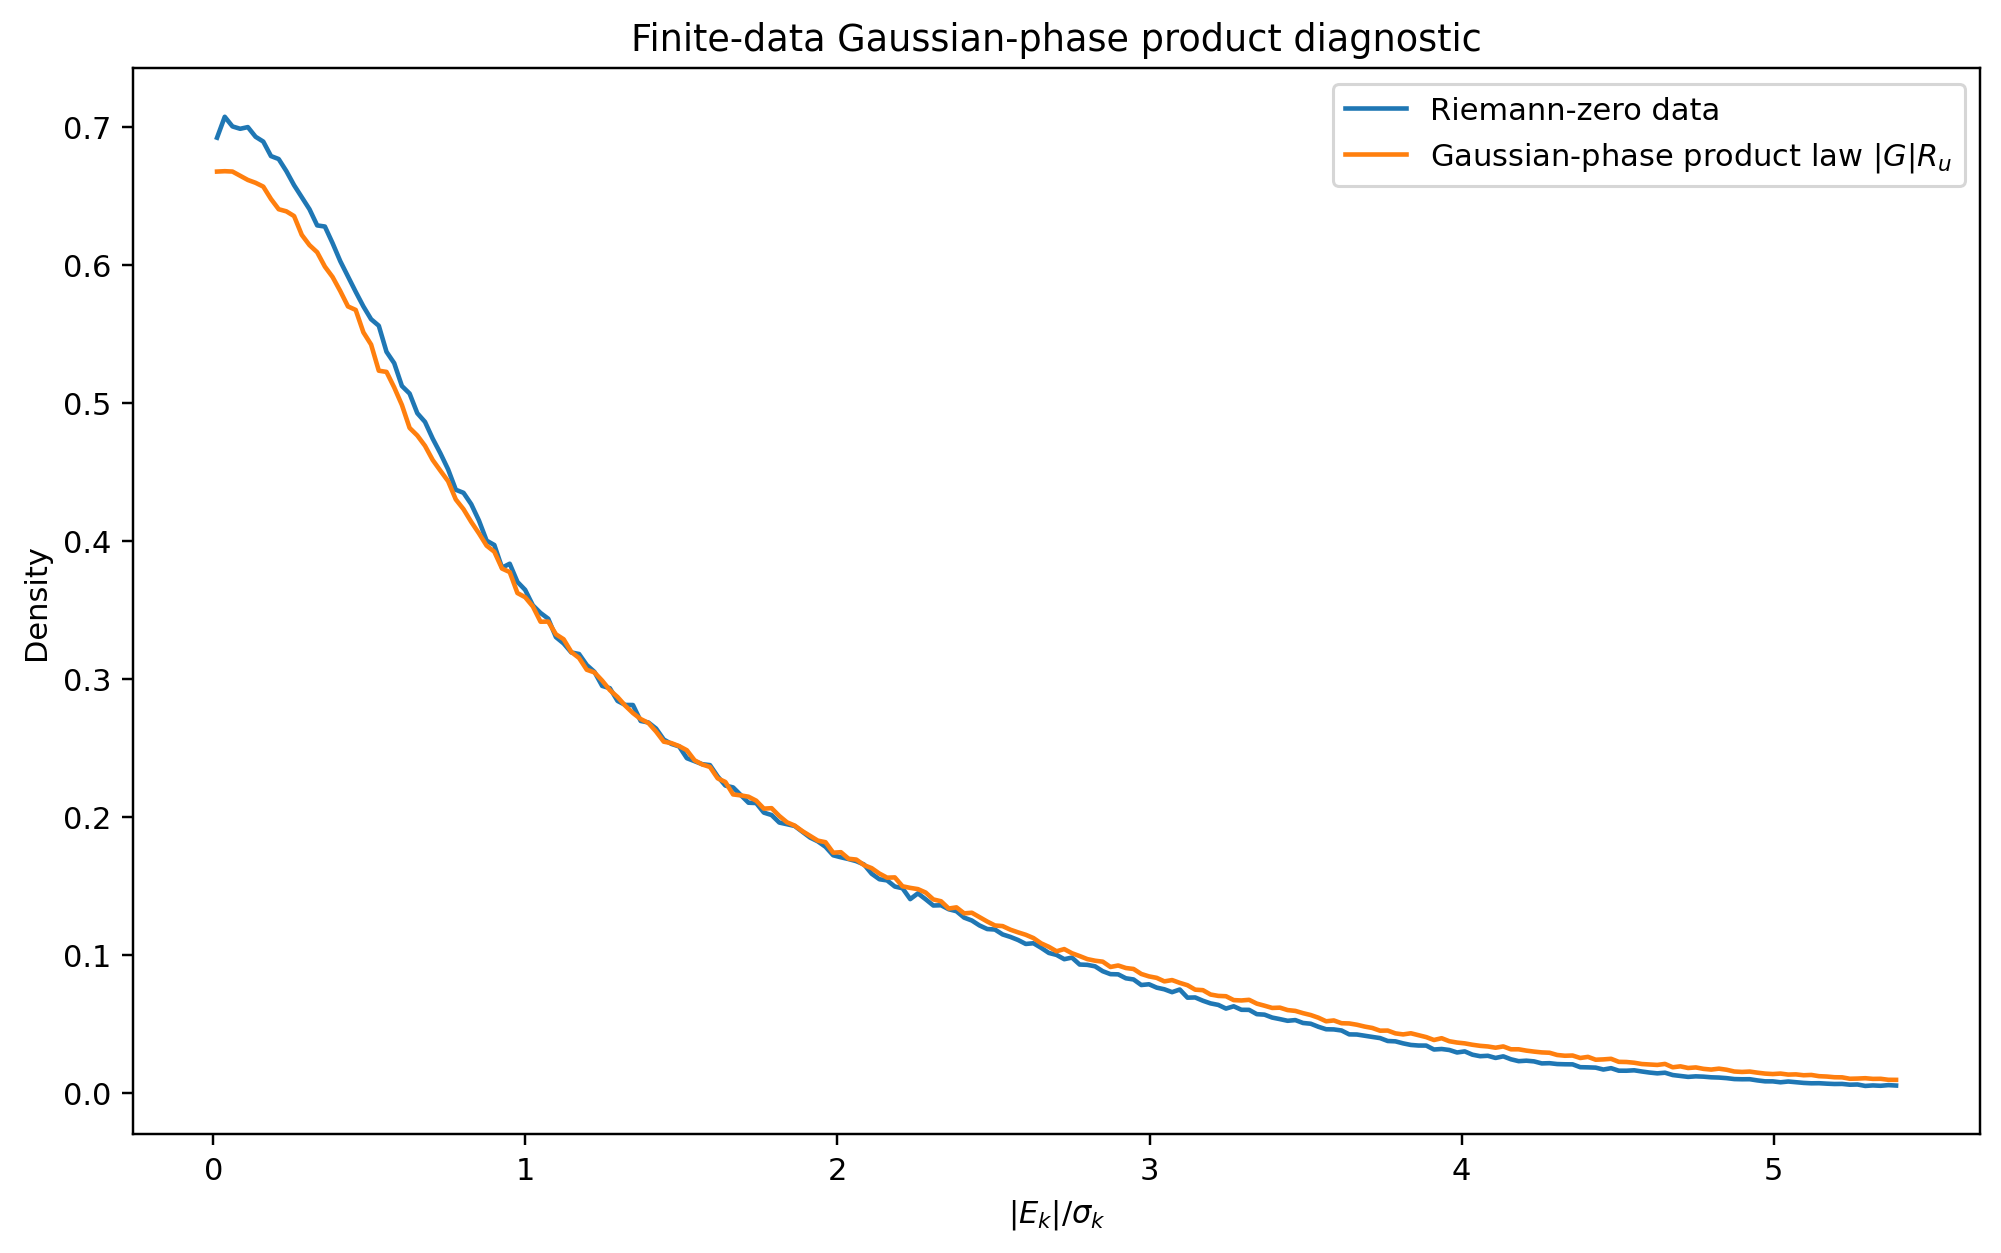
\includegraphics[width=0.92\textwidth]{Fig1.png}
\caption{Finite-height distribution of the normalized zero--clock exponential
residual compared with the Gaussian--phase product reference law.}
\label{fig:gaussian_phase_product}
\end{figure}


\section{The deterministic four-phase shark-fin law}

\begin{definition}[Shark-fin law]
Let $m_{\Torus^4}$ denote Haar probability measure on $\Torus^4$, and let
$\Theta=(\Theta_1,\ldots,\Theta_4)\sim m_{\Torus^4}$.  We denote by
$\RSF$ the probability law of
\[
 R_{\mathrm{SF}}(\Theta)
 :=\left|e^{i\Theta_1}+e^{i\Theta_2}+e^{i\Theta_3}+e^{i\Theta_4}\right|.
\]
Its radial density is
\[
 p_{\mathrm{SF}}(r)
 =
 r\int_0^\infty J_0(rx)J_0(x)^4\,x\,dx,
 \qquad 0<r<4,
\]
and its first two moments are
\[
 \E\RSF=1.799092479842851\ldots,
 \qquad
 \E\RSF^2=4.
\]
\end{definition}

\begin{lemma}[Two-chord representation]
\label{lem:twochord}
Let
\[
 A=e^{i\alpha_2}-e^{i\alpha_1},
 \qquad
 B=e^{i\beta_2}-e^{i\beta_1},
\]
with four Haar-uniform phase coordinates.  Then
\[
 |A-B|\overset d=\RSF.
\]
\end{lemma}

\begin{proof}
\[
 A-B=e^{i\alpha_2}+e^{i(\alpha_1+\pi)}
     +e^{i(\beta_2+\pi)}+e^{i\beta_1}.
\]
Adding $\pi$ preserves Haar measure.
\end{proof}

\begin{theorem}[Deterministic four-phase criterion]
\label{thm:four_phase_criterion}
If
\[
 (f_1(k),f_2(k),f_3(k),f_4(k))\bmod2\pi
\]
is equidistributed in $\Torus^4$ and
\[
 \Delta_k=
 (e^{if_1(k)}-e^{if_2(k)})
 -(e^{if_3(k)}-e^{if_4(k)}),
\]
then
\[
 |\Delta_k|\Longrightarrow\RSF.
\]
\end{theorem}

\begin{proof}
Equidistribution means that the empirical measures of
\((f_1(k),\ldots,f_4(k))\bmod2\pi\) converge weakly to Haar probability
measure on \(\Torus^4\).  The map
\[
 (\theta_1,\theta_2,\theta_3,\theta_4)
 \longmapsto
 \left|(e^{i\theta_1}-e^{i\theta_2})-(e^{i\theta_3}-e^{i\theta_4})\right|
\]
is continuous.  The continuous mapping theorem therefore gives convergence
of the empirical radial laws to the Haar law of this two-chord expression,
which is \(\RSF\) by Lemma~\ref{lem:twochord}.
\end{proof}

\begin{theorem}[Deterministic four-phase shark-fin law along zeta zeros]
\label{thm:hlawka_shark}
Let $u=(u_1,u_2,u_3,u_4)\in\R^4$ have rationally independent coordinates and define
\[
 \Delta_k(u)=
 (e^{iu_1\gamma_k}-e^{iu_2\gamma_k})
 -(e^{iu_3\gamma_k}-e^{iu_4\gamma_k}).
\]
Then
\[
 |\Delta_k(u)|\Longrightarrow\RSF.
\]
\end{theorem}

\begin{proof}
By multidimensional Weyl's criterion \cite{Weyl1916}, the phase vector is equidistributed in $\Torus^4$ iff
\[
 \frac1N\sum_{k\le N}e^{i(m\cdot u)\gamma_k}\to0
\]
for every $m\in\Z^4\setminus\{0\}$.  Rational independence gives $m\cdot u\ne0$.  Hlawka's theorem \cite{Hlawka1975} supplies the one-dimensional Weyl limit for every fixed nonzero real frequency.  Apply Theorem~\ref{thm:four_phase_criterion}.
\end{proof}

\begin{remark}[Reference law and zeta-zero realization]
The law \(\RSF\) is classical as a four-phase radial law.  Its occurrence in
Theorem~\ref{thm:hlawka_shark}, however, is a deterministic zeta-zero
realization.  The four phases are fixed functions of \(\gamma_k\), and their
Haar product structure is obtained from Hlawka's theorem and Weyl's criterion.
In the short-walk literature the same density is derived from four independent
uniform steps \cite{BorweinEtAl2012,BorweinStraubWan2013,McCrorie2021}; that random-walk construction is not an assumption of the
zeta-zero theorem.  The noteworthy point here is that the same radial law
arises without assuming or knowing any random-walk structure of the zeros.  The distinct index dynamics are quantified in Proposition~\ref{prop:phase_window_rigidity} and in Remark~\ref{rem:measured_index_corr}.
\end{remark}

\begin{proposition}[Phase-window rigidity]
\label{prop:phase_window_rigidity}
Fix \(J\ge1\) and \(u=(u_1,\ldots,u_J)\in\R^J\), and put
\[
 \Theta_k(u):=(u_1\gamma_k,\ldots,u_J\gamma_k)\bmod2\pi.
\]
Let \(r_N\) be any nonnegative integer sequence with \(r_N=o(\log N)\), and let
\(K_N\) be uniform on \(\{k_0,\ldots,N-r_N\}\).  For any fixed metric
\(d_{\Torus^J}\) induced by the Euclidean metric on \(\R^J\),
\begin{equation}
 \max_{0\le j\le r_N}
 d_{\Torus^J}\!\left(\Theta_{K_N+j}(u),\Theta_{K_N}(u)\right)
 \longrightarrow0
\label{eq:phase_window_rigidity}
\end{equation}
in \(L^1\), hence in probability.

In particular, for a rationally independent four-frequency vector \(u\), let
\(R_k(u):=|\Delta_k(u)|\).  If \(j_N\le r_N\), then
\[
 (R_{K_N}(u),R_{K_N+j_N}(u))
 \Longrightarrow
 (\RSF,\RSF),
\]
where the two coordinates on the right are the same random variable, and
\begin{equation}
 \Corr(R_{K_N}(u),R_{K_N+j_N}(u))\longrightarrow1.
\label{eq:radial_local_corr}
\end{equation}
Thus the one-point limiting law is $\RSF$, whereas the index process is
locally rigid on every \(o(\log N)\) window.
\end{proposition}

\begin{proof}
By zero ordering,
\[
 \max_{0\le j\le r_N}
 |\gamma_{K_N+j}-\gamma_{K_N}|
 =
 \gamma_{K_N+r_N}-\gamma_{K_N}.
\]
Writing \(M_N=N-r_N-k_0+1\), telescoping gives
\begin{align*}
 \E\!\left(\gamma_{K_N+r_N}-\gamma_{K_N}\right)
 &=
 \frac1{M_N}
 \sum_{k=k_0}^{N-r_N}(\gamma_{k+r_N}-\gamma_k)\\
 &=
 \frac{
 \sum_{m=N-r_N+1}^{N}\gamma_m
 -
 \sum_{m=k_0}^{k_0+r_N-1}\gamma_m
 }{M_N}\\
 &\le
 \frac{r_N\gamma_N}{M_N}.
\end{align*}
Riemann--von Mangoldt inversion gives \(\gamma_N\asymp N/\log N\), hence the last
quantity is \(O(r_N/\log N)=o(1)\).  Since quotient distance on the torus is no
larger than Euclidean distance of representatives,
\[
 \max_{0\le j\le r_N}
 d_{\Torus^J}\!\left(\Theta_{K_N+j}(u),\Theta_{K_N}(u)\right)
 \le
 \|u\|_2\bigl(\gamma_{K_N+r_N}-\gamma_{K_N}\bigr),
\]
which proves \eqref{eq:phase_window_rigidity} in \(L^1\).

For the four-phase observable, the map
\[
 \theta\longmapsto
 \left|
 (e^{i\theta_1}-e^{i\theta_2})
 -(e^{i\theta_3}-e^{i\theta_4})
 \right|
\]
is Lipschitz on \(\Torus^4\).  Therefore
\(R_{K_N+j_N}(u)-R_{K_N}(u)\to0\) in probability, uniformly for
\(j_N\le r_N\).  The variables are bounded by \(4\), so the convergence also holds
in every fixed \(L^p\).  Replacing the full prefix $\{k\le N\}$ by $\{k\le N-r_N\}$ does
not change the limiting empirical law, since $r_N=o(N)$.  Therefore
Theorem~\ref{thm:hlawka_shark} gives
\(R_{K_N}(u)\Rightarrow\RSF\), whose variance is positive; the \(L^2\) convergence
of the difference then gives \eqref{eq:radial_local_corr}.
\end{proof}


\begin{remark}[Measured index correlations and the finite-height regime]
\label{rem:measured_index_corr}
Proposition~\ref{prop:phase_window_rigidity} is asymptotic in the height, and
its limiting correlation-one regime is not numerically visible at the heights
of the present dataset.  It is useful to record the finite-height behaviour,
both because it gives a direct diagnostic of the indexed dynamics and because
it must not be read as contradicting the proposition.

For \(u=(1,\sqrt2,\sqrt3,\sqrt5)\) and \(R_k(u)=|\Delta_k(u)|\), the empirical
index correlations over the full dataset are
\begin{center}
\small
\begin{tabular}{@{}lrrrr@{}}
\toprule
lag & 1 & 2 & 3 & 4\\
\midrule
\(\Corr(R_k,R_{k+\mathrm{lag}})\)
& \(0.8911\) & \(0.6520\) & \(0.3557\) & \(0.0796\)\\
\midrule
lag & 5 & 7 & 10 & 20\\
\midrule
\(\Corr(R_k,R_{k+\mathrm{lag}})\)
& \(-0.1245\) & \(-0.2800\) & \(-0.2619\) & \(-0.1329\)\\
\bottomrule
\end{tabular}
\end{center}
The full table of twenty lags is supplied in
\path{outputs/shark_fin_index_correlations.txt}.

The exact phase increment is
\[
 \Theta_{k+1}(u)-\Theta_k(u)
 =u\,(\gamma_{k+1}-\gamma_k)\pmod{2\pi}.
\]
For scale comparison only, replace the fluctuating zero gap by the local clock
spacing \(d_k^{\rm clk}=2\pi/L_k\).  The corresponding clock-scale phase
increment is
\begin{equation}
 \delta\Theta_k^{\rm clk}(u):=\frac{2\pi}{L_k}(u_1,\ldots,u_4).
\label{eq:phase_step}
\end{equation}
At the top of the dataset,
\[
 \|\delta\Theta_k^{\rm clk}(u)\|_2
 \approx \sqrt{11}\times0.5192\approx1.72
 \quad\hbox{radians}.
\]
Thus the small-displacement regime used asymptotically in
Proposition~\ref{prop:phase_window_rigidity} is not yet a small one-step scale
here.  The fastest coordinate has a clock-scale \(2\pi\)-revolution length
\(L/u_{\max}\approx12.10/2.236\approx5.41\) indices, comparable with the
observed first sign change between lags \(4\) and \(5\).  This comparison is a
finite-height diagnostic, not a pointwise approximation asserting that
individual zeta-zero gaps equal their clock spacings.

The negative lobe is equally informative: the correlation reaches about
\(-0.280\) near lag \(7\) and then returns toward zero with oscillation.
Independent repeated realizations of the classical four-step construction
would have zero correlation between distinct samples; the classical one-point
law itself does not prescribe an index process.  The measured profile instead
shows deterministic oscillatory index structure, consistent with the
quasi-periodic geometry of the four fixed phases.  This concerns the indexed
process, not the one-point law: by Theorem~\ref{thm:hlawka_shark}, the limiting
empirical law of \(R_k(u)\) is \(\RSF\), while
Proposition~\ref{prop:phase_window_rigidity} proves local rigidity in the
asymptotic \(o(\log N)\) regime.  Equality of the one-point law with a classical
radial distribution is therefore not an independence statement across zero
indices.
\end{remark}



\subsection{Fixed-frequency numerical audit}
\label{subsec:fixed_frequency_audit}

Using all \(2{,}001{,}052\) ordinates and
\[
 u=(1,\sqrt2,\sqrt3,\sqrt5),
\]
the fixed-frequency four-phase observable gives:
\begin{center}
\begin{tabular}{@{}lr@{}}
\toprule
Quantity & Value\\
\midrule
sample count & \(2{,}001{,}052\)\\
mean radius, data & \(1.799094395840\)\\
exact shark-fin mean & \(1.799092479843\)\\
mean deviation & \(1.915997\times10^{-6}\)\\
second moment, data & \(4.000000861075\)\\
exact second moment & \(4\)\\
second-moment deviation & \(8.610750\times10^{-7}\)\\
approx.\ KS shape diagnostic vs \(8\times10^6\) reference draws
& \(3.822\times10^{-4}\)\\
\bottomrule
\end{tabular}
\end{center}

The two moment deviations are the cleaner diagnostics.  For orientation only,
an i.i.d.\ four-step sample of this size would have standard error
\[
 \sqrt{\frac{4-(\E\RSF)^2}{N}}=6.18\times10^{-4}
\]
for the sample mean; this is not used as a sampling model for the deterministic
zeta-zero sequence.

The Landau--Gonek comparison used here is unconditional and does not rely on
a finite verification of RH.  Away from prime-power logarithmic resonances,
the Landau--Gonek explicit formula supplies the natural comparison scale for
the corresponding finite-height Weyl sums \cite{Gonek1985,Gonek1993}.
Odlyzko identifies \texttt{zeros6.txt} as the first \(2{,}001{,}052\)
zeros \cite{OdlyzkoZeros}.  Platt--Trudgian \cite{PlattTrudgian2021} has a
different and independent role: their rigorous verification of RH through
height \(3\cdot10^{12}\) lies far above the largest ordinate in the present
table, about \(1.13\times10^6\), so every nontrivial zero in the height range
used here lies on the critical line.  Thus the critical-line status of the
entire numerical range is independently certified; it is not an assumption
behind the Landau--Gonek comparison.  These finite checks are provenance
checks only and are not used in the proof of
Theorem~\ref{thm:hlawka_shark}.

The second moment has an exact decomposition.  With
\(\epsilon=(+1,-1,-1,+1)\),
\[
 |\Delta_k(u)|^2
 =
 4+2\sum_{1\le a<b\le4}\epsilon_a\epsilon_b
 \cos\!\bigl((u_a-u_b)\gamma_k\bigr),
\]
so
\[
 \frac1N\sum_{k\le N}|\Delta_k(u)|^2-4
\]
is exactly a linear combination of six fixed-frequency Weyl sums.

\medskip\noindent\textbf{Nonresonance check.}
For \(u=(1,\sqrt2,\sqrt3,\sqrt5)\), the four coordinates are rationally
independent and every difference \(u_a-u_b\) is a nonzero algebraic number.
If such a difference were \(m\log p\), then \(e^{u_a-u_b}=p^m\) would be
algebraic, contradicting Lindemann--Weierstrass; see \cite{Baker1990}.
Thus none of the six difference frequencies is a prime-power logarithmic
resonance.  The full-data comparison is shown in Figure~\ref{fig:fixed_shark_fin}.

\begin{figure}[htbp]
\centering
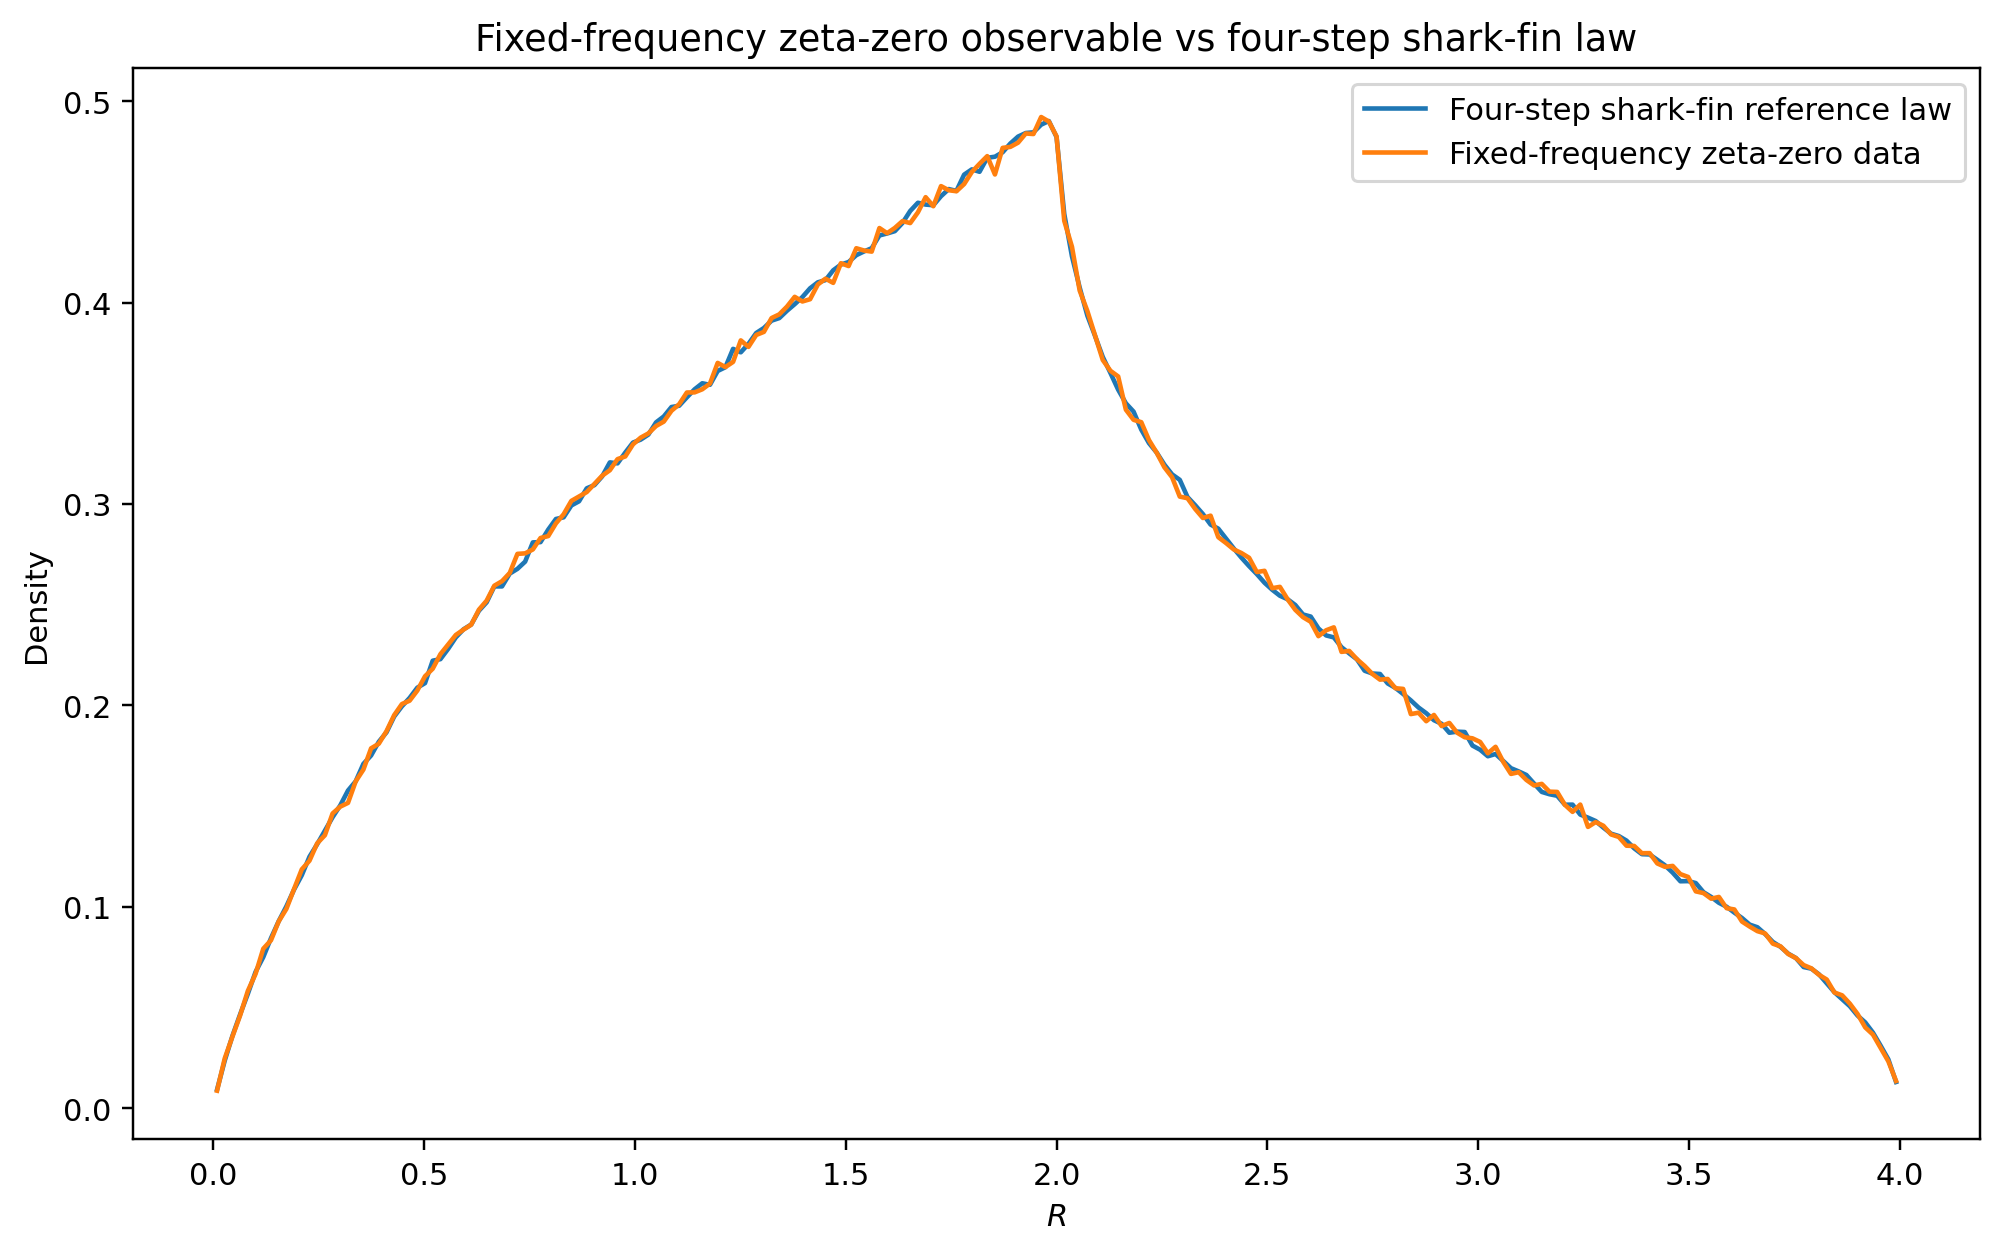
\includegraphics[width=0.94\textwidth]{Fig2.png}
\caption{Fixed-frequency four-phase zeta-zero observable for
\(u=(1,\sqrt2,\sqrt3,\sqrt5)\), compared with an independent simulation of
the classical four-step radial reference law.}
\label{fig:fixed_shark_fin}
\end{figure}

\subsection{Lagged \texorpdfstring{\(q_k=k\log k\)}{qk=k log k} diagnostic}

Define
\[
 q_k=k\log k,\qquad
 z_k=e^{i\gamma_kq_k},\qquad
 w_k=e^{i\tau_kq_k},
\]
and
\[
 \Delta_{1,1}(k)=(z_{k+1}-z_k)-(w_{k+1}-w_k).
\]
This uses adjacent indices and a frequency depending on $k$.  Starting at $k=3$ leaves $2{,}001{,}049$ evaluable terms from the full $2{,}001{,}052$-entry arrays; no shorter input dataset is used.  It is therefore not an instance of Theorem~\ref{thm:hlawka_shark}.  Its raw diagnostics are:

\begin{center}
\begin{tabular}{@{}lr@{}}
\toprule
Quantity & Value\\
\midrule
sample count & $2,001,049$\\
mean radius, data & $1.80020415689$\\
exact shark-fin mean & $1.799092479843$\\
mean deviation & $1.111677e-03$\\
second moment, data & $4.004212467$\\
exact second moment & $4$\\
second-moment deviation & $4.212467e-03$\\
normalized-shape KS diagnostic & $5.41e-04$\\
\bottomrule
\end{tabular}
\end{center}

The shape is close to the four-step radial profile, but the raw first and second moments show a finite systematic offset.  Normalizing each sample by its own empirical mean removes a scale parameter and therefore makes the corresponding KS statistic a shape diagnostic, not an exact distribution-free two-sample test.

The source ordinate table is quoted with accuracy within $4\times10^{-9}$.  Since $q_k=k\log k$, this accuracy is amplified in the phase.  At the top of the dataset the worst-case phase uncertainty from that quoted bound is of order $0.1$ radian.  This lagged high-frequency diagnostic is therefore tied to the supplied ordinate table and is not used as an asymptotic theorem check.  Figure~\ref{fig:lagged_shark_fin} shows its normalized radial profile.



\begin{figure}[htbp]
\centering
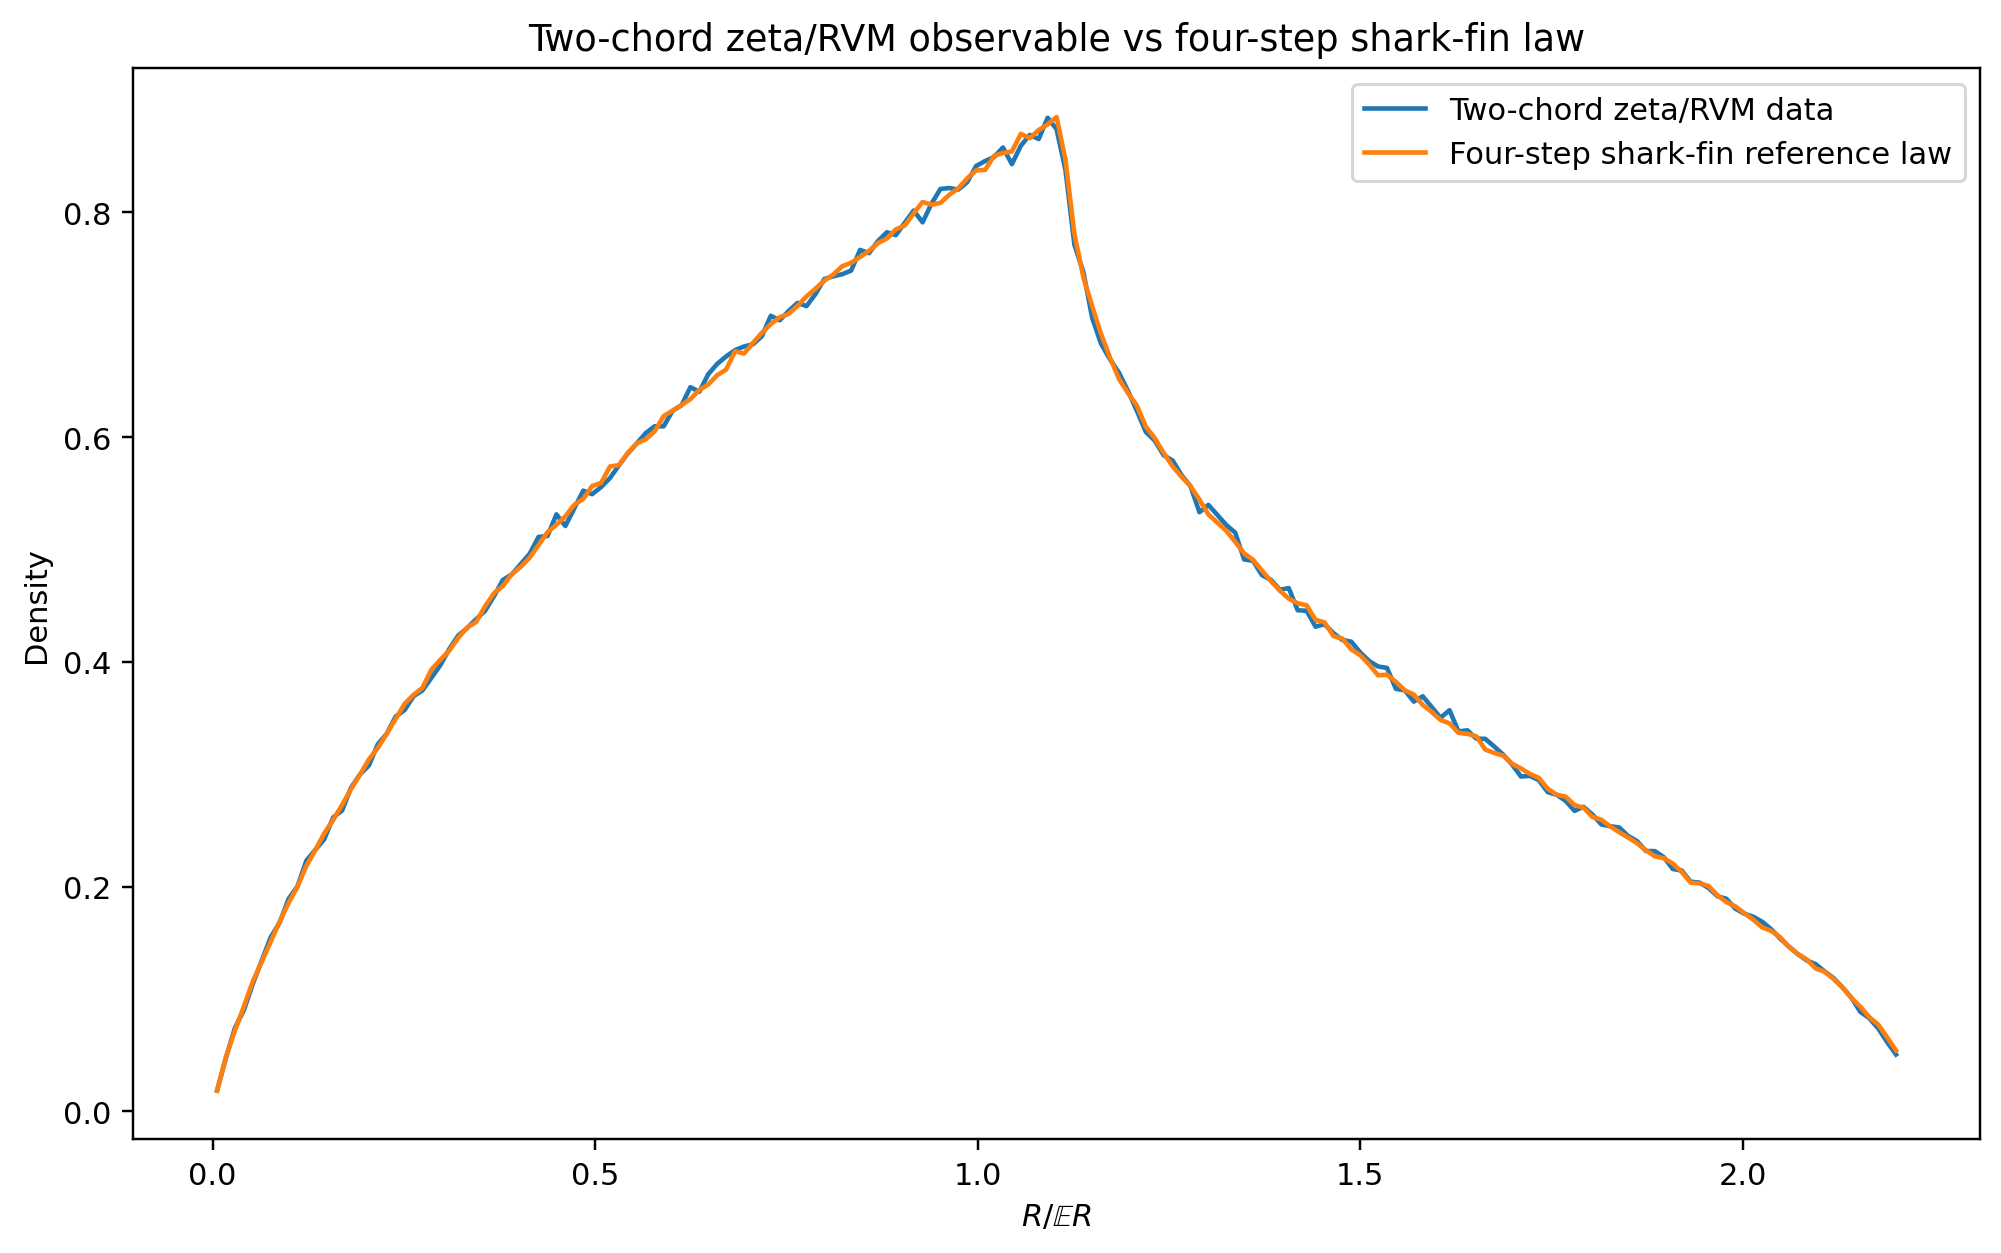
\includegraphics[width=0.94\textwidth]{Fig3.png}
\caption{Lagged two-chord zeta/Riemann--von Mangoldt observable compared with
the four-step radial reference law after the normalization described in the
text.  This is a diagnostic for the supplied finite table, not an instance of
Theorem~\ref{thm:hlawka_shark}.}
\label{fig:lagged_shark_fin}
\end{figure}


\section{Adjacent-zero diagonal limit and growing-window rigidity}
\label{sec:growing_window}

The ordering of the zeros produces a rigidity statement below the scale treated by Kargin's
separated-index covariance theorem.  The proof uses only the one-point prefix law, slow variation
of the smooth clock and normalization, and the monotonicity $\gamma_{k+j}\ge\gamma_k$.

\begin{theorem}[Growing-window collapse and decoupling]
\label{thm:growing_window}
Let $r_N$ be a nonnegative integer sequence satisfying
\begin{equation}
 r_N=o\!\left(\sqrt{\log\log N}\right).
\label{eq:r_window}
\end{equation}
Let $K_N$ be uniform on
\[
 \{k_0,\ldots,N-r_N\}.
\]
Then the following statements hold unconditionally.

\begin{enumerate}[label=\textup{(\roman*)}]
\item
\begin{equation}
 \max_{0\le j\le r_N}|X_{K_N+j}-X_{K_N}|
 \longrightarrow0
\label{eq:window_rigidity}
\end{equation}
in probability.

\item For every fixed integer $s\ge0$,
\begin{equation}
 (X_{K_N},X_{K_N+1},\ldots,X_{K_N+s})
 \Longrightarrow
 (G,G,\ldots,G),
\label{eq:fixed_window_diagonal}
\end{equation}
where all coordinates on the right are the same standard Gaussian variable.  Moreover, for every
fixed $j\ge1$,
\begin{equation}
 \Corr(X_{K_N},X_{K_N+j})\longrightarrow1.
\label{eq:fixed_lag_corr}
\end{equation}

\item For every fixed integer $s\ge0$, every $J\ge1$, and every $u\in\mathcal U_J$ from
Theorem~\ref{thm:samezero},
\begin{equation}
 \left(
 X_{K_N},\ldots,X_{K_N+s},
 (u_1\gamma_{K_N},\ldots,u_J\gamma_{K_N})\bmod2\pi
 \right)
 \Longrightarrow
 (G,\ldots,G,\Theta),
\label{eq:window_phase_decoupling}
\end{equation}
where $\Theta$ is Haar-uniform on $\Torus^J$ and independent of $G$.
\end{enumerate}
\end{theorem}

\begin{proof}
Fix $\epsilon\in(0,1)$.  On the bulk event $K_N\ge\epsilon N$, whose probability tends to
at least $1-\epsilon$, the clock relation and the mean-value theorem give, uniformly for
$0\le i<j\le r_N$,
\begin{equation}
 \tau_{K_N+j}-\tau_{K_N+i}
 \ll
 \frac{j-i}{\log N}.
\label{eq:bulk_clock_increment}
\end{equation}
The normalization is slowly varying on the same range:
\begin{equation}
 \max_{0\le i,j\le r_N}
 \left|\frac{\sigma_{K_N+i}}{\sigma_{K_N+j}}-1\right|
 =o(1).
\label{eq:bulk_sigma_ratio}
\end{equation}
Also
\begin{equation}
 \min_{0\le j\le r_N}\sigma_{K_N+j}
 \asymp
 \frac{\sqrt{\log\log N}}{\log N}.
\label{eq:bulk_sigma_size}
\end{equation}
Hence, by \eqref{eq:r_window},
\begin{equation}
 b_N(\epsilon):=
 \max_{\substack{0\le i<j\le r_N\\K_N\ge\epsilon N}}
 \frac{\tau_{K_N+j}-\tau_{K_N+i}}
      {\min_{0\le m\le r_N}\sigma_{K_N+m}}
 \longrightarrow0.
\label{eq:bulk_error}
\end{equation}

For $0\le i<j\le r_N$, zero ordering gives
\begin{equation}
 \sigma_{K_N+j}X_{K_N+j}
 -
 \sigma_{K_N+i}X_{K_N+i}
 \ge
 -(\tau_{K_N+j}-\tau_{K_N+i}).
\label{eq:ordered_sigma_X}
\end{equation}
Taking $i=0$ and $j=r_N$,
\begin{equation}
 X_{K_N+r_N}
 \ge
 \frac{\sigma_{K_N}}{\sigma_{K_N+r_N}}X_{K_N}
 -b_N(\epsilon).
\label{eq:endpoint_lower}
\end{equation}
The variables $X_{K_N}$ are tight by Lemma~\ref{lem:prefix}.  The shifted variables \(X_{K_N+r_N}\) have the same limiting marginal.  Indeed,
for every fixed moment order \(q\), shifting a prefix by \(r_N=o(N)\) changes its
average by at most
\[
 \frac{2r_N}{N}\max_{k\le N+r_N}|X_k|^q
 \ll \frac{r_N\log^q(2N)}{N}=o(1),
\]
because here \(r_N=o(\sqrt{\log\log N})\) and Lemma~\ref{lem:pointwiseX} applies.
Thus \(X_{K_N+r_N}\) is tight and also converges to \(N(0,1)\).  By \eqref{eq:bulk_sigma_ratio}--\eqref{eq:endpoint_lower},
the negative part of $X_{K_N+r_N}-X_{K_N}$ tends to zero in probability.

Consider a weakly convergent subsequence of the endpoint pair and write its limit as
$(Y_1,Y_2)$.  Portmanteau applied to
$\{(x,y):y-x<-\delta\}$ gives $Y_2\ge Y_1$ almost surely.  Both coordinates have the
same $N(0,1)$ law.  More generally, if two real random variables have the same law and
$Y_2\ge Y_1$ almost surely, then they are equal almost surely: for every rational $q$,
\[
 \{Y_1>q\}\subseteq\{Y_2>q\}
\]
with equal probabilities, and
\[
 \{Y_1<Y_2\}
 =
 \bigcup_{q\in\mathbb Q}\{Y_1\le q<Y_2\}
\]
is null.  Thus every subsequential endpoint limit is $(G,G)$, and
\begin{equation}
 X_{K_N+r_N}-X_{K_N}\longrightarrow0
\label{eq:endpoint_collapse}
\end{equation}
in probability.

For an intermediate $j\le r_N$, \eqref{eq:ordered_sigma_X} with $(i,j)=(0,j)$ gives
a lower bound by $X_{K_N}-o_{\Prob}(1)$, uniformly in $j$.  Applying the same inequality
to $(i,j)=(j,r_N)$ gives an upper bound by
$X_{K_N+r_N}+o_{\Prob}(1)$, uniformly in $j$.  Together with
\eqref{eq:endpoint_collapse}, this proves \eqref{eq:window_rigidity}.  Since $\epsilon$
was arbitrary, the bulk restriction disappears.

For fixed $s$, \eqref{eq:fixed_window_diagonal} follows from
\eqref{eq:window_rigidity}, Lemma~\ref{lem:prefix}, and Slutsky.  The uniform fourth
moment bound in Lemma~\ref{lem:prefix}, applied also to every fixed shift, gives uniform
integrability of the squares and cross-products; therefore the second mixed moments pass
to the limit and yield \eqref{eq:fixed_lag_corr}.

Finally Theorem~\ref{thm:samezero} is unchanged if the uniform prefix is truncated by
$r_N=o(N)$ indices.  For fixed $s$, \eqref{eq:window_rigidity} gives
\[
 (X_{K_N},\ldots,X_{K_N+s},\Theta_{K_N})
 =
 (X_{K_N},\ldots,X_{K_N},\Theta_{K_N})+o_{\Prob}(1),
\]
where
\[
 \Theta_{K_N}:=(u_1\gamma_{K_N},\ldots,u_J\gamma_{K_N})\bmod2\pi.
\]
Slutsky and Theorem~\ref{thm:samezero} prove \eqref{eq:window_phase_decoupling}.
\end{proof}

\subsection{Relation to Kargin's separated-index theorem}
\label{subsec:kargin_position}

Kargin's bivariate theorem \cite[Thm.~1.2]{Kargin2013} assumes
\[
 k'-k\asymp(\log k)^\beta,\qquad \beta>0,
\]
and gives a bivariate Gaussian limit with correlation \((1-\beta)_+\).
Consequently, it does not contain the bounded-gap case \(\beta=0\).  Since
\[
 \sqrt{\log\log N}=o\!\bigl((\log N)^\beta\bigr)
 \qquad(\beta>0\ \text{fixed}),
\]
the range \(r_N=o(\sqrt{\log\log N})\) of
Theorem~\ref{thm:growing_window} lies strictly below every separation scale
covered by Kargin's joint theorem.

\medskip\noindent\textbf{What is new here beyond Kargin.}
The additional conclusions established here are:
\begin{enumerate}
\item for every fixed \(r\ge1\),
\[
 (X_{K_N},X_{K_N+r})\Longrightarrow(G,G),
\]
so the full first-order joint law is obtained at \(\beta=0\);
\item the fixed-gap statement is strengthened to simultaneous collapse over
every growing window \(r_N=o(\sqrt{\log\log N})\);
\item the resulting bounded-gap block inherits the same-zero phase
decoupling \eqref{eq:window_phase_decoupling}; and
\item the proof uses zero ordering, the smooth-clock scale, tightness, and
the same-law order argument rather than an extension of Kargin's
positive-power prime-sum moment calculation.
\end{enumerate}
Thus the new content relative to \cite{Kargin2013} is the joint diagonal law
at the excluded \(\beta=0\) edge, its growing-window extension, and its
phase-decoupled form.

\medskip\noindent\textbf{Why the prime-sum input does not fill the gap.}
Kargin's covariance calculation invokes Bourgade's mesoscopic estimate
\cite{Bourgade2010}.  Bourgade's result is a statement about a prime sum,
and its bounded-shift regime is compatible with the formal value \(1\) at
the \(\beta=0\) scale.  It is not a theorem about
\(\Corr(X_k,X_{k+r})\), nor does it provide a joint law for bounded index
separation.  Transport from that analytic input to zero fluctuations in
Kargin's paper uses the joint-moment and comparison machinery formulated
under the hypothesis \(\beta>0\).  The present theorem supplies a different
route to the bounded-gap joint law and makes no claim that the prime-sum
estimate alone already contained that result.

\begin{remark}[Critical-scale interpretation]
\label{rem:critical_window_interpretation}
Theorem~\ref{thm:growing_window} proves collapse below
$\sqrt{\log\log N}$.  If the canonical increment
\[
 D_k:=\sqrt{\log\log\tau_k}\,(X_{k+1}-X_k)
\]
has a nondegenerate local limit, then this is also the natural scale at which accumulated
microscopic increments can become order one.  This observation motivates the scale but is
not used as a proof of optimality of \eqref{eq:r_window}.
\end{remark}

\section{Exact bridge from displacement increments to nearest-neighbor gaps}

Put
\[
 L_k:=\log\frac{\tau_k}{2\pi},
 \qquad
 d_k^{\mathrm{clk}}:=\frac{2\pi}{L_k}.
\]
The clock equation and the mean-value theorem give
\[
 \tau_{k+1}-\tau_k=d_k^{\mathrm{clk}}(1+o(1)).
\]
Write \(\sigma(T)=\sqrt{2\log\log T}/\log(T/(2\pi))\).  Direct
differentiation gives
\[
 \frac{\sigma'(T)}{\sigma(T)}
 =
 O\!\left(\frac1{T\log(T/(2\pi))}\right).
\]
Since \(\tau_{k+1}-\tau_k=O(1/L_k)\), another application of the
mean-value theorem yields
\[
 \frac{|\sigma_{k+1}-\sigma_k|}{d_k^{\mathrm{clk}}}
 =O\!\left(\frac{\sigma_k}{\tau_kL_k}\right)=o(1).
\]
Moreover, Lemma~\ref{lem:pointwiseX} gives
$|X_{k+1}|\ll\log(2+k)$.  Hence
\begin{equation}
 \frac{(\sigma_{k+1}-\sigma_k)X_{k+1}}{d_k^{\mathrm{clk}}}
 =o(1)
\label{eq:sigma_gap_error}
\end{equation}
pointwise as $k\to\infty$.  In particular this error is negligible in
probability and in every fixed local second-moment calculation used below.
Using the exact decomposition
\[
 \sigma_{k+1}X_{k+1}-\sigma_kX_k
 =
 \sigma_k(X_{k+1}-X_k)
 +(\sigma_{k+1}-\sigma_k)X_{k+1},
\]
we obtain
\begin{align}
 \frac{\gamma_{k+1}-\gamma_k}{d_k^{\mathrm{clk}}}
 &=
 \frac{\tau_{k+1}-\tau_k}{d_k^{\mathrm{clk}}}
 +
 \frac{\sigma_k}{d_k^{\mathrm{clk}}}
 (X_{k+1}-X_k)
 +o_{\Prob}(1)\\
 &=
 1+
 \frac{\sqrt{2\log\log\tau_k}}{2\pi}
 (X_{k+1}-X_k)
 +o_{\Prob}(1).
\label{eq:gapbridge}
\end{align}

Thus the normalized gap is governed by
\begin{equation}
 D_k:=\sqrt{\log\log\tau_k}\,(X_{k+1}-X_k),
\label{eq:Dcanonical}
\end{equation}
not by the first-order limit of either $X_k$ separately.  Equation~\eqref{eq:gapbridge} can be written
\begin{equation}
 G_k^{\mathrm{gap}}
 =
 1+\frac{\sqrt2}{2\pi}D_k+o_{\Prob}(1).
\label{eq:D_gap_dictionary}
\end{equation}
Thus the microscopic displacement increment and the normalized
nearest-neighbor gap are related, to first order, by the explicit affine map
\(D\mapsto 1+D/(\sqrt2\pi)\).  Nonnegativity of the normalized gap corresponds
at leading order to the boundary
\[
 D=-\sqrt2\,\pi=-4.44288294\ldots.
\]
This is an asymptotic dictionary rather than a pointwise support statement,
because the remainder in \eqref{eq:D_gap_dictionary} is \(o_{\Prob}(1)\).

\begin{corollary}[Transfer of any eventual microscopic gap law]
\label{cor:D_machine}
Assume that the prefix law of \(D_k\) converges to a moment-determinate
probability law \(\nu_D\), that every fixed moment converges, that the
corresponding fixed absolute moments are uniformly bounded, and that the
algebraic polynomials are dense in \(L^2(\nu_D)\).  Then for every $J\ge1$ and Lebesgue-almost every $u\in\R^J$,
\begin{equation}
 \left(
 D_k,
 (u_1\gamma_k,\ldots,u_J\gamma_k)\bmod2\pi
 \right)
 \Longrightarrow
 (D,\Theta),
\label{eq:D_phase_decoupling}
\end{equation}
where $D\sim\nu_D$, $\Theta$ is Haar-uniform on $\Torus^J$, and the two factors are independent.
\end{corollary}

\begin{proof}
Apply Proposition~\ref{prop:machine} with $\Psi_k=D_k$.
\end{proof}

\begin{remark}
Corollary~\ref{cor:D_machine} does not supply the law of $D_k$; its hypotheses contain precisely
the missing microscopic spacing information.  Its content is a transfer statement: once such a
law is established, no new twisted-moment calculation is required to decouple it from almost every
fixed arithmetic phase vector.
\end{remark}

\begin{proposition}[Variance-correlation relation at the microscopic scale]
\label{prop:varcorr}
Let
\[
 \mathcal I_n=\{a_n,a_n+1,\ldots,b_n\},
 \qquad a_n\longrightarrow\infty,
\]
be consecutive index windows, and let $K_n$ be uniform on
$\mathcal I_n^-:=\{a_n,\ldots,b_n-1\}$.  Choose any representative
$k_n\in\mathcal I_n$ and put
\[
 \ell_n:=\log\log\tau_{k_n}.
\]
Assume
\begin{equation}
 \sup_{k\in\mathcal I_n}
 \left|\frac{L_k}{L_{k_n}}-1\right|\longrightarrow0,
 \qquad
 \delta_n:=
 \sup_{k\in\mathcal I_n}
 \left|\log\log\tau_k-\ell_n\right|
 \longrightarrow0.
\label{eq:local_window_constancy}
\end{equation}
All variances and correlations below are taken with respect to the uniform
law of $K_n$.  Write
\[
 G_{K_n}^{\mathrm{gap}}
 :=
 \frac{\gamma_{K_n+1}-\gamma_{K_n}}{2\pi/L_{K_n}},
 \qquad
 c_n:=\frac{\sqrt{2\ell_n}}{2\pi},
\]
and set
\[
 V_{0,n}:=\Var(X_{K_n}),
 \qquad
 V_{1,n}:=\Var(X_{K_n+1}),
 \qquad
 \rho_{1,n}:=\Corr(X_{K_n},X_{K_n+1}).
\]
Suppose
\[
 V_{0,n}\longrightarrow v,
 \qquad
 V_{1,n}\longrightarrow v,
 \qquad
 \E X_{K_n}^2+\E X_{K_n+1}^2=O(1)
\]
for some $v>0$, and assume the shifted-window variance imbalance is negligible
on the microscopic scale:
\begin{equation}
 \ell_n\bigl(\sqrt{V_{0,n}}-\sqrt{V_{1,n}}\bigr)^2\longrightarrow0.
\label{eq:local_variance_balance}
\end{equation}
Then
\begin{equation}
 \Var\bigl(G_{K_n}^{\mathrm{gap}}\bigr)
 =
 \frac{v\,\ell_n}{\pi^2}\,(1-\rho_{1,n})
 \,\bigl(1+o(1)\bigr)+o(1).
\label{eq:finite_varcorr}
\end{equation}
Consequently, if the normalized gap variance tends to a finite nonzero limit
$V$, then
\[
 1-\rho_{1,n}
 =
 \frac{\pi^2V}{v\,\ell_n}
 +o\!\left(\frac1{\ell_n}\right).
\]
The asymptotic unit-variance case is $v\to1$; equation
\eqref{eq:finite_varcorr} is also the finite-height algebraic relation used
in the numerical reconstructions below.
\end{proposition}

\begin{remark}[Second moment in place of variance]
In the numerical reconstructions the measured second moment
$\langle X^2\rangle$ is used in place of the variance.  Over the full prefix,
$\langle X\rangle=-3.48\times10^{-7}$ and hence
$\langle X\rangle^2=1.2\times10^{-13}$.  On the top-window set of
$250{,}001$ zero indices used below, the corresponding square of the mean is
$3.06\times10^{-11}$.  Both are far below every digit reported in the variance
comparisons.
\end{remark}

\begin{proof}
By \eqref{eq:gapbridge} and \eqref{eq:sigma_gap_error}, for
$k\in\mathcal I_n^-$,
\begin{equation}
 G_k^{\mathrm{gap}}
 =1+\frac{\sqrt{2\log\log\tau_k}}{2\pi}\,(X_{k+1}-X_k)+\eta_{k,n}.
\label{eq:gap_local_exact}
\end{equation}
Here the rate can be read directly from the same clock estimates, without
strengthening \eqref{eq:gapbridge}.  Since
$M'(T)=L(T)/(2\pi)$ and $M''(T)=1/(2\pi T)$, the mean-value theorem gives
\[
 \frac{\tau_{k+1}-\tau_k}{2\pi/L_k}-1
 =O\!\left(\frac1{\tau_kL_k^2}\right).
\]
Moreover, the estimate preceding \eqref{eq:sigma_gap_error} and
Lemma~\ref{lem:pointwiseX} give
\[
 \frac{(\sigma_{k+1}-\sigma_k)X_{k+1}}{2\pi/L_k}
 =O\!\left(\frac{\sigma_k\log(2+k)}{\tau_kL_k}\right)
 =O\!\left(\frac{\sqrt{\log\log\tau_k}}{k}\right),
\]
where the last step uses $\tau_k\asymp k/\log k$ and $L_k\asymp\log k$.
Consequently, uniformly for $k\ge a_n$,
\[
 \eta_{k,n}=O\!\left(\frac{\sqrt{\log\log\tau_k}}{k}\right).
\]
By \eqref{eq:local_window_constancy},
$\log\log\tau_k=\ell_n+o(1)$ uniformly on $\mathcal I_n$, so
\begin{equation}
 \sqrt{\ell_n}\,
 \sup_{k\in\mathcal I_n^-}|\eta_{k,n}|
 =O\!\left(\frac{\ell_n}{a_n}\right)=o(1).
\label{eq:eta_L2_rate}
\end{equation}
Thus the additive remainder is small at the rate needed for a local variance
calculation; no supremum bound on $X_{k+1}-X_k$ is used.

Factor the slowly varying coefficient as
\begin{equation}
 \frac{\sqrt{2\log\log\tau_k}}{2\pi}
 =c_n\bigl(1+\theta_{k,n}\bigr),
 \qquad
 \theta_{k,n}
 :=\sqrt{\frac{\log\log\tau_k}{\ell_n}}-1.
\label{eq:coeff_factorization}
\end{equation}
Since $\delta_n\to0$ and $\ell_n\to\infty$,
\begin{equation}
 \Theta_n:=\sup_{k\in\mathcal I_n}|\theta_{k,n}|
 =O\!\left(\frac{\delta_n}{\ell_n}\right).
\label{eq:theta_uniform}
\end{equation}
Write
\[
 A_n:=c_n(X_{K_n+1}-X_{K_n}),
 \qquad
 R_n:=\theta_{K_n,n}A_n+\eta_{K_n,n}.
\]
The bounded local second moments imply
$\E A_n^2=O(\ell_n)$.  Hence
\[
 \|\theta_{K_n,n}A_n\|_2
 \le \Theta_n\|A_n\|_2
 =O\!\left(\frac{\delta_n}{\sqrt{\ell_n}}\right),
\]
while \eqref{eq:eta_L2_rate} gives
$\sqrt{\ell_n}\,\|\eta_{K_n,n}\|_2\to0$.  Therefore
\begin{equation}
 \sqrt{\ell_n}\,\|R_n\|_2\longrightarrow0.
\label{eq:R_L2_rate}
\end{equation}
Since $\Var(A_n)^{1/2}\le\|A_n\|_2=O(\sqrt{\ell_n})$,
Cauchy--Schwarz yields
\begin{equation}
 \bigl|\Var(1+A_n+R_n)-\Var(A_n)\bigr|
 \le
 2\Var(A_n)^{1/2}\Var(R_n)^{1/2}+\Var(R_n)
 =o(1).
\label{eq:cross_term}
\end{equation}
This is the required second-moment control: the coefficient error is handled
in $L^2$ and the additive clock error has an explicit rate.

It remains to evaluate the main variance.  Exactly,
\begin{align}
 \Var(A_n)
 &=c_n^2\bigl(V_{0,n}+V_{1,n}
       -2\rho_{1,n}\sqrt{V_{0,n}V_{1,n}}\bigr)\\
 &=\frac{\ell_n}{\pi^2}\sqrt{V_{0,n}V_{1,n}}\,(1-\rho_{1,n})
 +\frac{\ell_n}{2\pi^2}
  \bigl(\sqrt{V_{0,n}}-\sqrt{V_{1,n}}\bigr)^2.
\label{eq:varA}
\end{align}
By \eqref{eq:local_variance_balance} the second term is $o(1)$, while
$\sqrt{V_{0,n}V_{1,n}}=v(1+o(1))$.  Combining
\eqref{eq:cross_term} and \eqref{eq:varA} proves
\eqref{eq:finite_varcorr}.
\end{proof}

\begin{remark}[Numerical verification of the window hypotheses]
For the top $250{,}000$ consecutive pairs used in
Section~\ref{subsec:adjacent_numerics}, take $\mathcal I$ to be the
$250{,}001$ supporting zero indices and $k_n$ its midpoint.  Directly from the
canonical data,
\[
 \sup_{k\in\mathcal I}\left|\frac{L_k}{L_{k_n}}-1\right|
 =0.005249,
 \qquad
 \sup_{k\in\mathcal I}
 \left|\log\log\tau_k-\log\log\tau_{k_n}\right|
 =0.004564.
\]
The variance-balance term in \eqref{eq:local_variance_balance} is
$2.45\times10^{-10}$.  With the midpoint coefficient,
\eqref{eq:varA} gives $0.167466$, against the measured normalized-gap variance
$0.167463$.  If instead the actual window-average coefficient
$\overline{\log\log\tau}=2.630452547$ is retained, the same local identity
gives $0.167462766$, compared with the measured $0.167462770$.  The difference
between the midpoint and averaged evaluations is exactly the finite-window
variation quantified above.
\end{remark}

\begin{remark}[What is and is not inherited from separated-index analysis]
At the prime-sum input level, Bourgade's bounded-shift estimate
\cite{Bourgade2010} is compatible with the formal \(\beta=0\) value that appears
inside Kargin's covariance calculation.  It is not a theorem about
\(\Corr(X_k,X_{k+r})\) at bounded index separation and it does not supply a
joint zero law.  Theorem~\ref{thm:growing_window} obtains that first-order joint
law by a different mechanism.  The nearest-neighbor spacing information then
survives only in the correction to the diagonal, at order
\(1/\sqrt{\log\log\tau_k}\) for displacement increments and
\(1/\log\log\tau_k\) for covariance.
\end{remark}


\subsection{Finite-height adjacent-zero audit}
\label{subsec:adjacent_numerics}

Using all $2{,}001{,}051$ consecutive pairs from the same ordinate table gives
\begin{center}
\begin{tabular}{@{}lr@{}}
\toprule
Quantity & Value\\
\midrule
$\langle X^2\rangle$, full prefix & $0.848888$\\
$\Corr(X_k,X_{k+1})$, full prefix & $0.246643$\\
$\langle D_k\rangle$, full prefix & $-1.64\times10^{-7}$\\
$\Var(D_k)$, full prefix & $3.278190$\\
$\min D_k$, full prefix & $-4.418684$\\
mean normalized gap & $0.999999$\\
variance normalized gap & $0.166075$\\
\bottomrule
\end{tabular}
\end{center}
The observed full-prefix minimum,
\[
 \min_k D_k=-4.418684,
\]
lies close to the leading-order boundary
\(-\sqrt2\pi=-4.442883\ldots\) furnished by
\eqref{eq:D_gap_dictionary}.  This is only a finite-height diagnostic: the
\(o_{\Prob}(1)\) remainder in the gap dictionary does not promote that
leading-order boundary to a pointwise support theorem.

For the top $250{,}000$ consecutive pairs extracted from the same full $2{,}001{,}052$-entry arrays, where the slowly varying coefficients are essentially
constant on the comparison scale, the reported marginal second moment is the
unweighted mean over the $250{,}001$ distinct zero indices supporting those
pairs:
\begin{center}
\begin{tabular}{@{}lr@{}}
\toprule
Quantity & Value\\
\midrule
median $\tau$ & $1.067435\times10^6$\\
mean $\log\log\tau$ & $2.630453$\\
mean marginal $\langle X^2\rangle$ & $0.856734$\\
empirical $\rho_1$ & $0.266593$\\
empirical normalized-gap variance & $0.167463$\\
$\rho_1$ using Wigner--GUE variance & $0.220025$\\
\bottomrule
\end{tabular}
\end{center}



\subsection{Finite-height GUE benchmark}
\label{subsec:gue_benchmark}

For the Wigner surmise in symmetry class GUE,
\begin{equation}
 V_{\mathrm{GUE}}^{\mathrm{W}}
 =
 \frac{3\pi}{8}-1
 =
 0.178097\ldots,
\label{eq:gue_wigner_var}
\end{equation}
whereas the GOE Wigner variance is
\[
 V_{\mathrm{GOE}}^{\mathrm{W}}
 =
 \frac4\pi-1
 =
 0.273240\ldots.
\]
Thus a variance near \(0.286\) must not be used as a GUE benchmark.
The finite-height comparison below uses throughout the GUE Wigner-surmise
value \(3\pi/8-1=0.178097\ldots\); the corresponding GOE value is
\(4/\pi-1=0.273240\ldots\).

Combining Proposition~\ref{prop:varcorr} with
\eqref{eq:gue_wigner_var}, and using asymptotic unit variance for \(X\),
gives the benchmark
\[
 \rho_1(T)
 \approx
 1-\frac{\pi^2V_{\mathrm{GUE}}^{\mathrm{W}}}{\log\log T}.
\]
Numerically,
\[
 \rho_1(10^6)=0.330583\ldots,\qquad
 \rho_1(10^{12})=0.470388\ldots,\qquad
 \rho_1(10^{30})=0.584970\ldots.
\]
If the measured finite-height second moment
\(\langle X^2\rangle=0.848888\) is inserted into the finite-height algebraic
relation, the corresponding values are \(0.211419\ldots\),
\(0.376111\ldots\), and \(0.511089\ldots\).

The empirical top-window normalized-gap variance \(0.167463\) is about
\(6.0\%\) below the Wigner--GUE benchmark \(0.178097\ldots\).  At the
present height this is recorded only as a finite-height discrepancy; no
convergence rate to a GUE spacing law is asserted.  Figure~\ref{fig:rho_corrected} shows the corresponding finite-height correlation benchmark.

\begin{figure}[htbp]
\centering
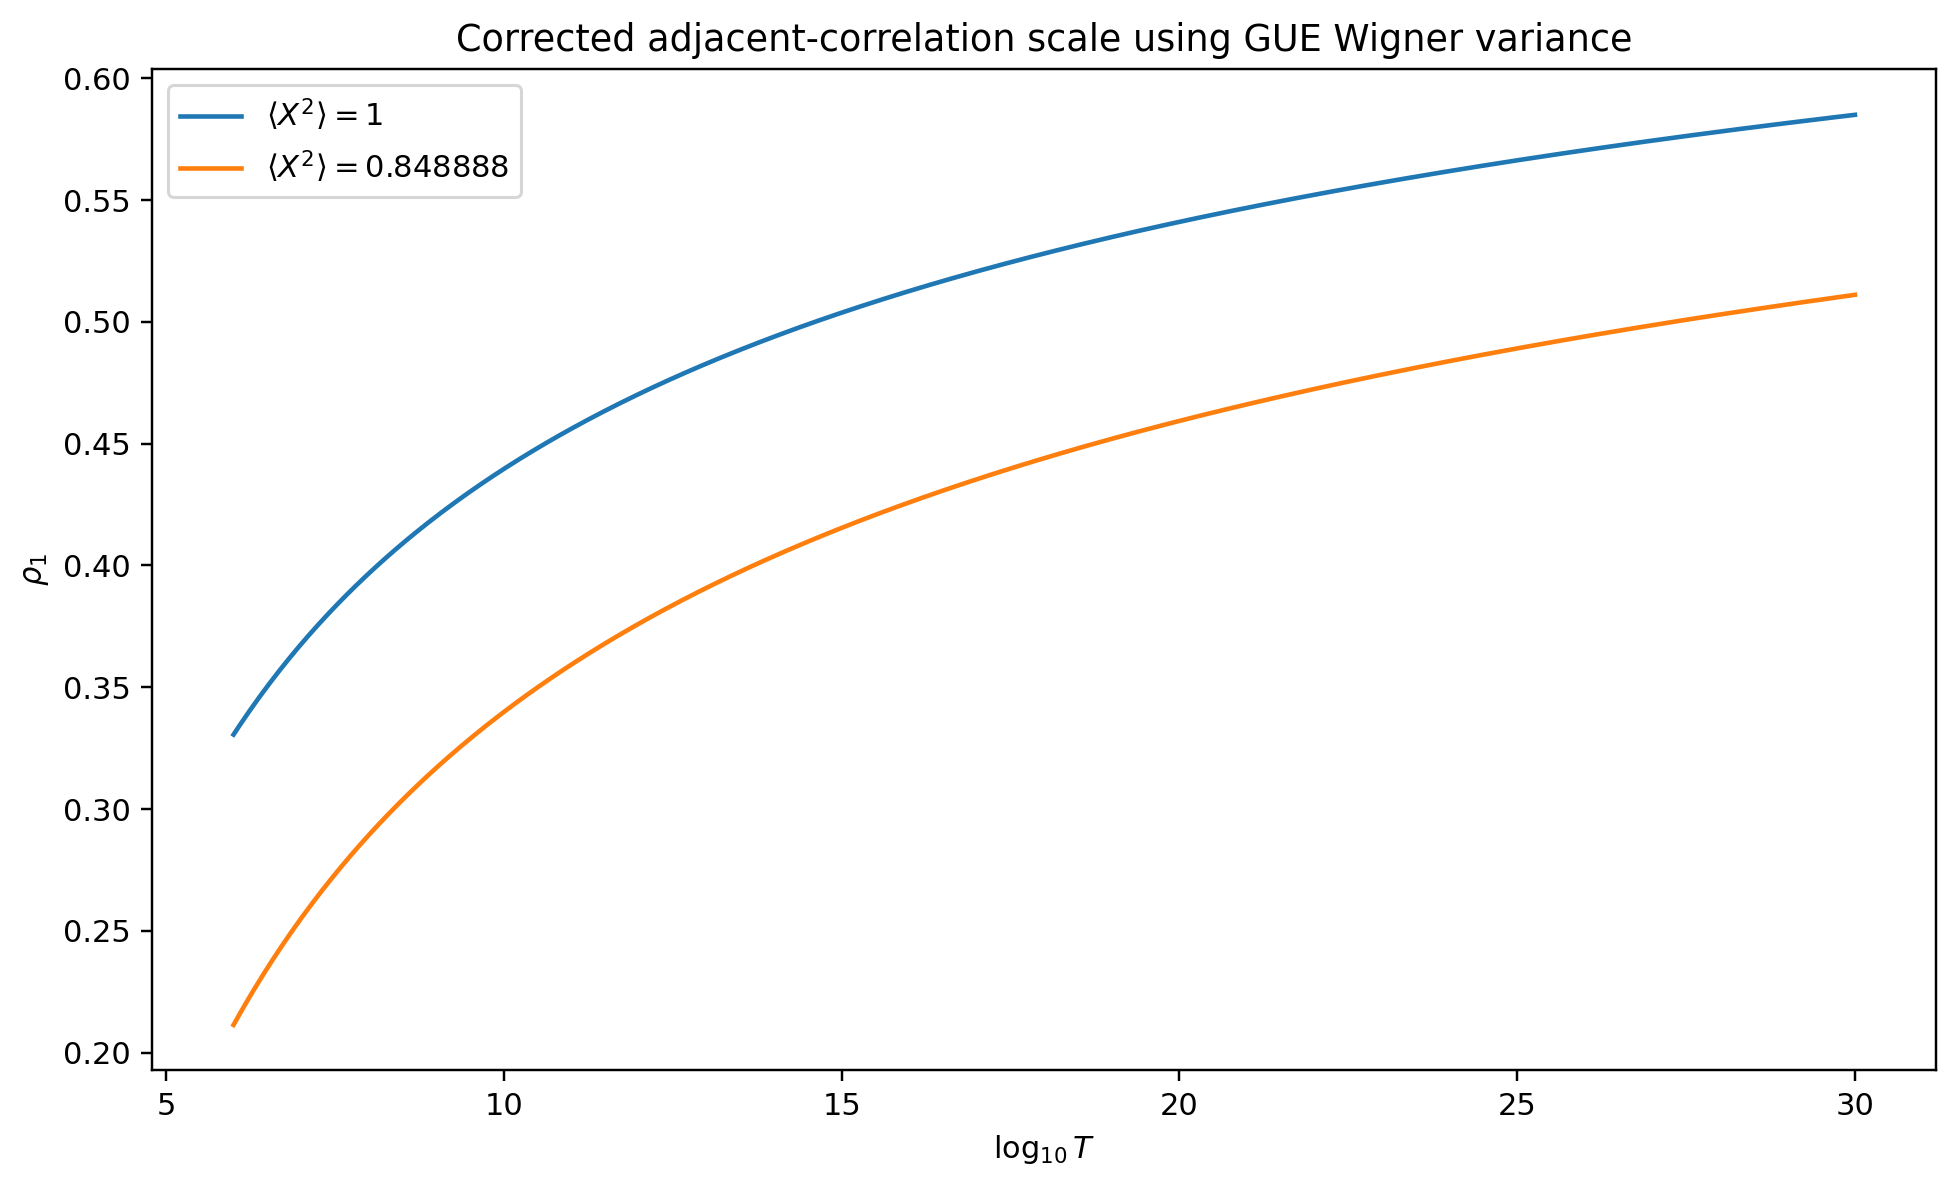
\includegraphics[width=0.92\textwidth]{Fig4.png}
\caption{Finite-height adjacent-correlation benchmark based on the corrected
Wigner--GUE spacing variance.  The two curves distinguish asymptotic unit
variance for \(X\) from the measured finite-height value \(0.848888\).}
\label{fig:rho_corrected}
\end{figure}

\section{Reproducibility and data provenance}

The zero ordinates used throughout this article are the first
\(2{,}001{,}052\) nontrivial Riemann-zeta ordinates published by
A.~M. Odlyzko in his public tables of zeta zeros \cite{OdlyzkoZeros}.
Odlyzko's table states an accuracy within \(4\times10^{-9}\) for this dataset.
The original plain-text table is included verbatim in the repository as
\path{data/zeros6.txt}, so the primary numerical source accompanies the
manuscript.  The file \path{data/zeross.bin} is the deterministic
double-precision binary encoding of those same ordinates used by the numerical
scripts.  The file \path{data/zLamb.bin} is deterministic derived data: it is
the smooth Riemann--von Mangoldt clock table computed from those ordinates and
the clock definition used in this paper.  These are the only three data files
required by the article.  Every numerical script first loads and verifies the full
$2{,}001{,}052$-entry \texttt{zeross.bin} and \texttt{zLamb.bin} arrays.
Any smaller sample count reported in a derived calculation is forced by the
mathematical observable itself---for example $N-1$ adjacent pairs, $N-j$
pairs at lag $j$, or an explicitly labelled top-height window---and never
comes from a separate or truncated input dataset.

\medskip\noindent\textbf{Reproducibility.}
All numerical tables and figures in this version are generated from the supplied
\texttt{zeross.bin} and \texttt{zLamb.bin} datasets by the scripts distributed with
the source archive.  The archive includes the generated CSV/TXT outputs and a SHA256
manifest.  No numerical value used in a theorem proof is taken from these computations.



\section{Use of AI tools}
\label{sec:ai}

Codex was used to check English usage and LaTeX formatting, to independently double-check
computations in Python, and to generate reproducibility scripts and figures. Claude was used
to identify potential inconsistencies and to suggest independent numerical checks. All
mathematical claims and numerical values included in the final manuscript were independently
audited against the stated definitions and cited literature by the author, who assumes sole
responsibility for the content.

\section{Literature position and scope}

For the fixed-frequency shark-fin theorem, Hlawka \cite{Hlawka1975} supplies
the one-dimensional Weyl tests and Weyl's criterion \cite{Weyl1916} assembles
the torus vector.  The resulting deterministic zeta-zero radial law coincides
with the classical four-step radial density studied in the short-walk literature
\cite{BorweinEtAl2012,BorweinStraubWan2013}.

The same-zero Gaussian--phase coupling is different from simply juxtaposing
Kargin's Gaussian marginal \cite{Kargin2013} and Hlawka's phase marginal
\cite{Hlawka1975}.  Closely related conditional same-index architectures do occur in
Çiçek--Gonek \cite{CicekGonek2024}: under RH and a zero-spacing hypothesis they combine
a Gaussian statistic attached to a zero with uniform distribution of the selected
ordinate subsequence.  Their twisted analysis includes sums in which an exponential
phase is weighted by powers of a Dirichlet polynomial.  The present result has a
different tradeoff: it is unconditional and applies to Lebesgue-almost every fixed
frequency vector, whereas Çiçek--Gonek obtain conditional results at prescribed
frequencies.  Their work builds on Çiçek's distribution theorem for the logarithm of
\(\zeta\) near nontrivial zeros \cite{Cicek2021}.  The metric sinc-kernel argument here
is therefore positioned as an unconditional almost-every-frequency decoupling
principle, not as the first appearance of a Gaussian-statistic/equidistribution
architecture.

The adjacent-zero theorem introduces a genuine two-zero object but shows that its first-order normalized displacement limit is completely degenerate:
\[
 (X_k,X_{k+1})\Rightarrow(G,G).
\]
The local spacing information begins only after magnifying the difference by $\sqrt{\log\log\tau_k}$.  Equivalently, the first nontrivial covariance information is the coefficient of
\[
 \frac1{\log\log\tau_k}
\]
in $1-\Corr(X_k,X_{k+1})$.

Unnormalized exponential sums at prime-power logarithms exhibit the classical Landau/von-Mangoldt resonance.  They do not produce exceptional frequencies for Hlawka's normalized equidistribution.  The genuinely unresolved twisted objects in the present metric argument are the displacement-weighted sums at prescribed arithmetic frequencies,
\[
 \frac1N\sum_{k\le N}X_k^\ell e^{iv\gamma_k},
 \qquad \ell\ge1,
\]
when $v$ is fixed in advance rather than chosen from the full-measure set supplied by Theorem~\ref{thm:metric}.

\section{Conclusion}

The main result is the same-zero theorem.  We also record an
adjacent-zero diagonal consequence of the ordinal viewpoint.

The same-zero theorem states that, for almost every fixed frequency vector, Kargin's normalized displacement becomes asymptotically independent of the torus phases of the same zero.  The metric sinc-kernel argument supplies the missing mixed cancellation and yields the Gaussian--phase product law.

The adjacent-zero diagonal consequence states that consecutive normalized displacements have the joint first-order limit $(G,G)$.  This identifies exactly why one-zero marginal information cannot determine nearest-neighbor spacing.  The spacing law resides in
\[
 \sqrt{\log\log\tau_k}\,(X_{k+1}-X_k),
\]
or equivalently in the $1/\log\log\tau_k$ correction to adjacent correlation.

Although the shark-fin law is an immediate consequence of Haar measure on
$\mathbb T^4$, the main objective of the present work is the same-zero
Gaussian--phase coupling and the metric independence theorem from which such
radial laws arise.

The four-frequency shark-fin result is retained as a deterministic
zeta-zero realization of the classical four-step radial law.  Its proof uses
Hlawka, Weyl, and the continuous two-chord map, and does not assume any
random-walk model for the zeros.  In the classical short-walk literature the
same radial density is obtained from a random-walk construction; the zeta-zero
result establishes it without that hypothesis.  It is noteworthy that this
classical radial law appears in a deterministic zeta-zero observable, where no
random-walk structure of the zeros is assumed or known.

\begin{thebibliography}{99}
\raggedright

\bibitem{Montgomery1973}
H.~L. Montgomery,
\textit{The pair correlation of zeros of the zeta function},
in \textit{Analytic Number Theory}, Proc. Sympos. Pure Math. \textbf{24},
Amer. Math. Soc., Providence, RI, 1973, 181--193.

\bibitem{RudnickSarnak1996}
Z.~Rudnick and P.~Sarnak,
\textit{Zeros of principal $L$-functions and random matrix theory},
Duke Math. J. \textbf{81} (1996), 269--322.

\bibitem{Hlawka1975}
E.~Hlawka,
\textit{\"Uber die Gleichverteilung gewisser Folgen, welche mit den Nullstellen der Zetafunktion zusammenh\"angen},
\"Osterreich. Akad. Wiss. Math.-Naturwiss. Kl. S.-B. II
\textbf{184} (1975), no.~8--10, 459--471.
\bibitem{Fujii1978}
A.~Fujii,
\textit{On the uniformity of the distribution of the zeros of the Riemann zeta function},
J. Reine Angew. Math. \textbf{302} (1978), 167--205.

\bibitem{FordZaharescu2005}
K.~Ford and A.~Zaharescu,
\textit{On the distribution of imaginary parts of zeros of the Riemann zeta function},
J. Reine Angew. Math. \textbf{579} (2005), 145--158.

\bibitem{FordMengZaharescu2017}
K.~Ford, X.~Meng, and A.~Zaharescu,
\textit{Simultaneous distribution of the fractional parts of Riemann zeta zeros},
Bull. Lond. Math. Soc. \textbf{49} (2017), no.~1, 1--9.
\bibitem{Kargin2013}
V.~Kargin,
\textit{On fluctuations of Riemann's zeta zeros},
Probab. Theory Related Fields \textbf{157} (2013), 575--604.
\\url{https://doi.org/10.1007/s00440-012-0465-9}.
\bibitem{Bourgade2010}
P.~Bourgade,
\textit{Mesoscopic fluctuations of the zeta zeros},
Probab. Theory Relat. Fields \textbf{148} (2010), 479--500.

\bibitem{Titchmarsh1986}
E.~C. Titchmarsh,
\textit{The Theory of the Riemann Zeta-Function},
2nd ed., revised by D.~R. Heath-Brown,
Oxford University Press, 1986.

\bibitem{BorweinEtAl2012}
J.~M. Borwein, A.~Straub, J.~Wan, and W.~Zudilin,
\textit{Densities of short uniform random walks},
with an appendix by Don Zagier,
Canad. J. Math. \textbf{64} (2012), no.~5, 961--990.
\\url{https://doi.org/10.4153/CJM-2011-079-2}.
\bibitem{BorweinStraubWan2013}
J.~M. Borwein, A.~Straub, and J.~Wan,
\textit{Three-step and four-step random walk integrals},
Experiment. Math. \textbf{22} (2013), no.~1, 1--14.
\\url{https://doi.org/10.1080/10586458.2013.748379}.
\bibitem{McCrorie2021}
J.~R. McCrorie,
\textit{Moments in Pearson's four-step uniform random walk problem and other applications of very well-poised generalized hypergeometric series},
Sankhya B \textbf{83} (2021), Suppl.~2, 244--281.
\\url{https://doi.org/10.1007/s13571-020-00230-1}.
\bibitem{Weyl1916}
H.~Weyl,
\textit{\"Uber die Gleichverteilung von Zahlen mod. Eins},
Math. Ann. \textbf{77} (1916), no.~3, 313--352.
\bibitem{Cicek2021}
F.~\c{C}i\c{c}ek,
\textit{On the logarithm of the Riemann zeta-function near the nontrivial zeros},
Trans. Amer. Math. Soc. \textbf{374} (2021), no.~8, 5995--6037.
\\url{https://doi.org/10.1090/tran/8426}.
\bibitem{CicekGonek2024}
F.~\c{C}i\c{c}ek and S.~M. Gonek,
\textit{The uniform distribution modulo one of certain subsequences of ordinates of zeros of the zeta function},
Math. Proc. Cambridge Philos. Soc. \textbf{176} (2024), no.~3, 593--608.
\\url{https://doi.org/10.1017/S0305004124000045}.
\bibitem{Gonek1985}
S.~M. Gonek,
\textit{A formula of Landau and mean values of $\zeta(s)$},
in \textit{Topics in Analytic Number Theory} (Austin, Tex., 1982),
Univ. Texas Press, Austin, TX, 1985, 92--97.
\bibitem{Gonek1993}
S.~M. Gonek,
\textit{An explicit formula of Landau and its applications to the theory of the zeta-function},
Contemp. Math. \textbf{143}, Amer. Math. Soc., Providence, RI, 1993, 395--413.
\bibitem{Baker1990}
A.~Baker,
\textit{Transcendental Number Theory},
2nd ed., Cambridge Mathematical Library, Cambridge University Press, 1990.

\bibitem{Bakan2001}
A.~G. Bakan,
\textit{Polynomial density in $L_p(\mathbb R,d\mu)$ and representation of all measures which generate a determinate Hamburger moment problem},
in M.~Lassonde (ed.), \textit{Approximation, Optimization and Mathematical Economics},
Physica, Heidelberg, 2001, 37--46.
\\url{https://doi.org/10.1007/978-3-642-57592-1\_3}.

\bibitem{PlattTrudgian2021}
D.~Platt and T.~S. Trudgian,
\textit{The Riemann hypothesis is true up to $3\cdot10^{12}$},
Bull. Lond. Math. Soc. \textbf{53} (2021), no.~3, 792--797.
\\url{https://doi.org/10.1112/blms.12460}.

\bibitem{Szego1975}
G.~Szeg\H{o},
\textit{Orthogonal Polynomials},
4th ed., Amer. Math. Soc. Colloq. Publ. \textbf{23},
Amer. Math. Soc., Providence, RI, 1975.


\bibitem{OdlyzkoZeros}
A.~M. Odlyzko,
\textit{Tables of zeros of the Riemann zeta function},
University of Minnesota, public numerical tables.
The table used here contains the first \(2{,}001{,}052\) zeros and is stated
to be accurate to within \(4\times10^{-9}\).
\url{https://www-users.cse.umn.edu/~odlyzko/zeta_tables/}.
Accessed 17 August 2026.

\end{thebibliography}

\end{document}
